%%%%%%%%%%%%%%%%%%%%%%% file template.tex %%%%%%%%%%%%%%%%%%%%%%%%%
%
% This is a general template file for the LaTeX package SVJour3
% for Springer journals.          Springer Heidelberg 2010/09/16
%
% Copy it to a new file with a new name and use it as the basis
% for your article. Delete % signs as needed.
%
% This template includes a few options for different layouts and
% content for various journals. Please consult a previous issue of
% your journal as needed.
%
%%%%%%%%%%%%%%%%%%%%%%%%%%%%%%%%%%%%%%%%%%%%%%%%%%%%%%%%%%%%%%%%%%%
%
% First comes an example EPS file -- just ignore it and
% proceed on the \documentclass line
% your LaTeX will extract the file if required
%\begin{filecontents*}{example.eps}
%!PS-Adobe-3.0 EPSF-3.0
%%BoundingBox: 19 19 221 221
%%CreationDate: Mon Sep 29 1997
%%Creator: programmed by hand (JK)
%%EndComments
%gsave
%newpath
%  20 20 moveto
%  20 220 lineto
%  220 220 lineto
%  220 20 lineto
%closepath
%2 setlinewidth
%gsave
%  .4 setgray fill
%grestore
%stroke
%grestore
%\end{filecontents*}
%
\RequirePackage{fix-cm}
\RequirePackage{amsmath}
%
%\documentclass{svjour3}                     % onecolumn (standard format)
%\documentclass[smallcondensed]{svjour3}     % onecolumn (ditto)
%\documentclass[smallextended]{svjour3}       % onecolumn (second format)
\documentclass[twocolumn]{svjour3}          % twocolumn
%
\smartqed  % flush right qed marks, e.g. at end of proof
%
\usepackage{graphicx}
%
\usepackage{mathptmx}      % use Times fonts if available on your TeX system
%
% insert here the call for the packages your document requires
\let\amalg\relax
\usepackage{amssymb,
mathtools,bm,extraipa,mathabx,graphicx,algorithm}
\usepackage{algpseudocode}
\usepackage{booktabs}
\usepackage{multirow}
\usepackage{url}

\usepackage{xcolor} % for colors

%\usepackage{latexsym}
% etc.
%
% please place your own definitions here and don't use \def but
% \newcommand{}{}

\newcommand{\fudge}{\fC}
\newcommand{\cc}{\mathcal{C}}
\newcommand{\dtf}{\textit{\doubletilde{f}}}
\newcommand{\cube}{[0,1]^d}
\newcommand{\rf}{\mathring{f}}
\newcommand{\rnu}{\mathring{\nu}}
\newcommand{\natm}{\naturals_{0,m}}
\newcommand{\wcS}{\widecheck{S}}
\newcommand{\tol}{\text{tol}}
\newcommand{\e}{\text{e}}
%\newcommand{\bvec}[1]{\boldsymbol{#1}}
\newcommand{\vect}[1]{\boldsymbol{\mathbf{#1}}}
\newcommand{\vx}{\vect{x}}
\newcommand{\vl}{\vect{l}}
\newcommand{\vI}{\vect{I}}
\newcommand{\vk}{\vect{k}}
\newcommand{\vw}{\vect{w}}
\newcommand{\vz}{\vect{z}}
\newcommand{\vt}{\vect{t}}
\newcommand{\dif}{\mathsf{d}}
\newcommand{\hf}{\hat{f}}
\newcommand{\hS}{\widehat{S}}
\newcommand{\tS}{\widetilde{S}}
\newcommand{\tf}{\widetilde{f}}
\newcommand{\fC}{\mathfrak{C}}
\newcommand{\homega}{\widehat{\omega}}
\newcommand{\wcomega}{\mathring{\omega}}
\newcommand{\vzero}{\vect{0}}
\newcommand{\integers}{\mathbb{Z}}
\newcommand{\naturals}{\mathbb{N}}
\newcommand{\ip}[3][{}]{\ensuremath{\left \langle #2, #3 \right \rangle_{#1}}}
\newcommand\iid{\stackrel{{\rm iid}}{\sim}}

\makeatletter
\newcommand{\ov}[1]{
  \m@th\overline{\mbox{#1}\raisebox{2mm}{}}
}
\newcommand{\absolute}[1]{\left\lvert#1\right\rvert}
\let\oldemptyset\emptyset
\let\emptyset\varnothing

\newcommand{\comment}[1]{{\color{cyan} #1 }}
% Insert the name of "your journal" with
% \journalname{myjournal}
%
\begin{document}

\title{Reliable error estimation for Sobol' indices\thanks{This work is supported by the CITiES project funded by the Agence Nationale de la Recherche (grant ANR-12-MONU-0020) and by the United States National Science Foundation (grant DMS-1522687).}
}
%\subtitle{Do you have a subtitle?\\ If so, write it here}

%\titlerunning{Short form of title}        % if too long for running head

\author{
        Llu\'{i}s Antoni Jim\'{e}nez Rugama \and  Laurent Gilquin}

%\authorrunning{Short form of author list} % if too long for running head

\institute{Llu\'{i}s Antoni Jim\'{e}nez Rugama \at
              Illinois Institute of Technology, Rettaliata Engineering Center, Room 208, 10 W 32st, Chicago, IL 60616 \\
\email{ljimene1@hawk.iit.edu}
           \and
           Laurent Gilquin \at
              Inria Grenoble - Rh\^{o}ne-Alpes, Inovall\'{e}e, 655 avenue de l'Europe, 38330 Montbonnot \\
\email{gilquin.laurent@inria.fr}   
}

\date{Received: date / Accepted: date}
% The correct dates will be entered by the editor


\maketitle

\begin{abstract}
In the field of sensitivity analysis, Sobol' indices are sensitivity measures widely used to assess the importance of inputs of a model to its output. The estimation of these indices is often performed {\color{purple}through} Monte Carlo or quasi-Monte Carlo methods. A notable method is the replication procedure that estimates first-order indices at a reduced cost in terms of number of model evaluations. 

An inherent practical problem of this estimation is how to quantify the number of model evaluations needed to ensure that estimates satisfy a desired error tolerance. This article addresses this challenge by proposing a reliable error bound for first-order and total effect Sobol' indices. Starting from the integral formula of the indices, the error bound is defined in terms of the discrete Walsh coefficients of the different integrands. 

We propose a sequential estimation procedure of Sobol' indices using the error bound as a stopping criterion. The sequential procedure combines Sobol' sequences with either Saltelli's strategy to estimate both first-order and total effect indices, or the replication procedure to estimate only first-order indices.

\keywords{Sobol' index \and error bound \and sequential method \and quasi-Monte Carlo}
% \PACS{PACS code1 \and PACS code2 \and more}
\subclass{49Q12 \and 62L12 \and 65R10}
\end{abstract}

%\section{Introduction}
%\label{intro}
%Your text comes here. Separate text sections with
%\section{Section title}
%\label{sec:1}
%Text with citations \cite{RefB} and \cite{RefJ}.
%\subsection{Subsection title}
%\label{sec:2}
%as required. Don't forget to give each section
%and subsection a unique label (see Sect.~\ref{sec:1}).
%\paragraph{Paragraph headings} Use paragraph headings as needed.
%\begin{equation}
%a^2+b^2=c^2
%\end{equation}

% For one-column wide figures use
%\begin{figure}
% Use the relevant command to insert your figure file.
% For example, with the graphicx package use
%  \includegraphics{example.eps}
% figure caption is below the figure
%\caption{Please write your figure caption here}
%\label{fig:1}       % Give a unique label
%\end{figure}
%
% For two-column wide figures use
%\begin{figure*}
% Use the relevant command to insert your figure file.
% For example, with the graphicx package use
%  \includegraphics[width=0.75\textwidth]{example.eps}
% figure caption is below the figure
%\caption{Please write your figure caption here}
%\label{fig:2}       % Give a unique label
%\end{figure*}
%
% For tables use
%\begin{table}
%% table caption is above the table
%\caption{Please write your table caption here}
%\label{tab:1}       % Give a unique label
%% For LaTeX tables use
%\begin{tabular}{lll}
%\hline\noalign{\smallskip}
%first & second & third  \\
%\noalign{\smallskip}\hline\noalign{\smallskip}
%number & number & number \\
%number & number & number \\
%\noalign{\smallskip}\hline
%\end{tabular}
%\end{table}

\section{Introduction}
\label{sec:1}

Let $f$ represent a deterministic numerical model in $[0,1]^d$, $d \geq 1$. Sensitivity measures, also known as Sobol' indices, are used to assess which inputs of $f$ are influential for the output. The normalized indices are scalars between $0$ and $1$ whose values are interpreted as follows: the closer to $1$ the more influential the index. Alternatively, they can be interpreted as the percentage of the variance explained by the inputs. Among all Sobol' indices one can distinguish first-order and total effect indices. The first measure the effect of a single input, while the second measure the effect of a single input plus all its interactions with other inputs.

When dealing with complex numerical models, analytical expressions of Sobol' indices are often inaccessible. In such cases, one must rely on an estimation of these indices. The original estimation procedure is due to Sobol' \cite{Sobol'}. However, this procedure requires several model evaluations which are usually expensive. Later on, Saltelli \cite{Saltelli} proposed strat\-egies to estimate sets of Sobol' indices at once through the use of a combinatorial formalisms. While elegant, these strat\-egies still require a large number of model evaluations.  A cost efficient alternative to estimate first-order indices was introduced in \cite{Mara}. This alternative, called the replication procedure, has recently been further studied  in \cite{Tissot} and generalized to the estimation of closed second-order indices.

A practical problem concerning the use of these methods is how to quantify the number of model evaluations required to ensure that Sobol' estimates are accurate enough. This article addresses this challenge by proposing a reliable error bound for Sobol' indices based on digital sequences. The error bound is defined in terms of the discrete Walsh coefficients of the integrands involved in the Sobol' indices definition. We propose a sequential estimation procedure of Sobol' indices using the error bound as our stopping criterion. The procedure operates under the assumption that all integrands lie inside a particular cone of functions (see \cite{HicJim}).

Firstly, Section \ref{sec:2} introduces Sobol' indices and reviews both Saltelli's strategy to estimate first-order and total effect Sobol' indices, and the replication procedure. Our main contribution is detailed in  Section \ref{sec:3}. There, we review the construction of the error bound proposed in \cite{HicJim} for the estimation of integrals based on digital sequences, and then we generalize it for Sobol' indices. Section \ref{sec:4} is devoted to analyze the cost in terms of model evaluations of our sequential estimation algorithm. It combines the error bound in Section \ref{sec:3} and either one of the two estimation procedures of Section \ref{sec:2}. We also discuss a potential improvement to estimate small first-order indices according to \cite{Owen}. Finally, examples and illustrations of our procedure are presented in Section \ref{sec:5}. 

\section{Background on Sobol' indices}
\label{sec:2}

\subsection{Definition of Sobol' indices}
\label{sec:2.1}
%We adopt the same notations introduced by Owen in \cite{Owen}. 
Denote by $\vx=(x_1,\dots,x_d)$ the vector of inputs of $f$. We assume that $f$ is in some subset of $\in \mathbb{L}^2(\cube)$ for which $f(\vx)$ is defined for all $\vx\in\cube$, and $\mathcal{D}=\{1,\dots,d\}$ the set of dimension indexes. %The uncertainty on $\vx$ is modeled by a random vector that we suppose uniformly distributed on $\cube$.
Let $u$ be a subset of $\mathcal{D}$, $-u$ its complement and $|u|$ its cardinality. Then, $\vx_u$ represents a point in $[0,1]^{|u|}$ with components $x_j, j \in u$. Given two points $\vx$ and $\vx'$, the hybrid point $\vw=(\vx_u:{\vx'}_{-u})$ is defined as $w_j=x_j$ if $j \in u$ and $w_j=x'_j$ if $j \notin u$.% and denote by $\mu$ and $\sigma^2$ the mean $\int_{\cube}f(\vx)d{\vx}$ and variance $\int_{\cube}(f(\vx)-\mu)^2d{\vx}$ of $f$.

The uncertainty on $\vx$ is modeled by a uniform random vector, namely $\vx \sim \mathcal{U}(\cube)$. The Hoeffding decomposition \cite{Hoeffding,Sobol'} of $f$ is:
\begin{equation}
f(\vx)=f_{\varnothing}+\sum \limits_{u \subseteq \mathcal{D}, u \neq \varnothing} f_u(\vx),
\label{anova}
\end{equation}
where:
\begin{align*}
f_{\varnothing} &= \mathbb{E}[f(\vx)]= \mu, \\
f_u(\vx) &= \int_{[0,1]^{|u|}} f(\vx) d{\vx}_{-u} - \sum \limits_{v \subsetneq u} f_v(\vx).
\end{align*}
Due to orthogonality, the variance of equation \eqref{anova} leads to the variance decomposition of $f$:
\[ \sigma^2 = \mathrm{Var}[f(\vx)] = \sum \limits_{u \subseteq \mathcal{D}, u \neq \varnothing} \sigma_u^2,\]
\[ \sigma_u^2=\int_{[0,1]^{|u|}} f_u(\vx)^2 d{\vx_u}.\]
From this decomposition, one can define the following two quantities:
\[\underline{\tau}_u^2 = \sum \limits_{v \subseteq u} \sigma_v^2, \qquad
\ov{$\tau$}_u^2 = \sum \limits_{v \cap u \neq \varnothing} \sigma_v^2, \qquad u \subseteq \mathcal{D}.\]

These two quantities $\underline{\tau}_u^2$ and $\ov{$\tau$}_u^2$ measure the importance of variables $\vx_u$: $\underline{\tau}_u^2$ quantifies the main effect of $\vx_u$, that is the effect of all interactions between variables in $\vx_u$, and $\ov{$\tau$}_u^2$ quantifies the main effect of $\vx_u$ plus the effect of all interactions between variables in $\vx_u$ and variables in $\vx_{-u}$.

Both $\underline{\tau}_u^2$ and $\ov{$\tau$}_u^2$ satisfy the following relations: $ 0 \leq  \underline{\tau}_u^2 \leq \ov{$\tau$}_u^2$ and $\underline{\tau}_u^2 = \sigma^2 - \ov{$\tau$}_{-u}^2$. These two measures are commonly found in the literature in their normalized form: $\underline{S}_u = \underline{\tau}_u^2 / \sigma^2$ is the closed $|u|$-order Sobol' index for inputs $u$, while $\ov{$S$}_u = \ov{$\tau$}_u^2 / \sigma^2$ is the total effect Sobol' index of order $|u|$.
\bigskip

%The problem of interest is the evaluation of first-order and total effect Sobol' indices.
In our framework, we are only interested in single input indices, namely $|u|=1$. The computation of the normalized indices is performed based on the following integral formulas for their numerators:
{\color{purple}(Lolo)
\begin{align}
\label{first.order}
\underline{\tau}_u^2  &= \int_{[0,1]^{2d}} \left(
f(\vx_u:{\vx'}_{-u})-f(\vx')\right)f(\vx)d\vx d{\vx'}, \\
\label{total.effect}
\ov{$\tau$}_u^2 &= \frac{1}{2}\int_{[0,1]^{d+1}}(f(\vx')-f(\vx_u:{\vx'}_{-u}))^2 d\vx_u d{\vx'}, \ u \in \mathcal{D},
\end{align}
}
while variance and mean of $f$ are evaluated as:
\begin{gather}
\begin{aligned}
\sigma^2 &= \int_{[0,1]^{d}} f(\vx)^2d{\vx} - \mu^2, \\
 \mu &= \int_{[0,1]^{d}} f(\vx) d{\vx},
\label{eq.sigma.mu}
\end{aligned}
\end{gather}
Usually the complexity of $f$ causes the solution of integrals \eqref{first.order}, (\ref{total.effect}) and (\ref{eq.sigma.mu}) to be intractable. In such cases, one can instead estimate these quantities.

\subsection{Estimation of Sobol' indices}
\label{sec:2.2}
In this section we review two Monte Carlo procedures for the estimation of Sobol' indices. A design is a point set $\mathcal{P}=\{\vx_i\}_{i=0}^{n-1}$ where each point is obtained by sampling each variable $x_j$ $n$ times. Each row of the design is a point $\vx_i$ in $[0,1]^d$ and each column of the design refers to samples of a variable $x_j$. Consider $\mathcal{P}=\{\vx_i\}_{i=0}^{n-1}$ and $\mathcal{P'}=\{{\vx'}_i\}_{i=0}^{n-1}$ two designs where $(\vx_i,{\vx'}_i) \iid \mathcal{U}([0,1]^{2d})$. One way to estimate the two quantities (\ref{first.order}) and (\ref{total.effect}) is via:
{\color{purple}(Lolo)
\begin{align}
\label{first.order.est}
\widehat{\underline{\tau}_u^2} &= \frac{1}{n} \sum \limits_{i=0}^{n-1} \left(f(\vx_{i,u}:{\vx'}_{i,-u})-f(\vx'_i)\right)f(\vx_i),\\
\label{total.effect.est}
\widehat{\ov{$\tau$}_u^2} &= \frac{1}{2n} \sum \limits_{i=0}^{n-1} (f({\vx'}_i) - f(\vx_{i,u}:{\vx'}_{i,-u}))^2, \qquad u \in \mathcal{D},
\end{align}
}
using for $\sigma^2$:
{\color{purple} (Lolo)
\begin{equation}
 \widehat{\sigma}^2 = \frac{1}{n-1} \sum \limits_{i=0}^{n-1} \left( f(\vx_i) - \widehat{\mu}\right)^2, \text{ with } \ \widehat{\mu} =  \frac{1}{n} \sum \limits_{i=0}^{n-1} f(\vx_i).
\label{mu.est}
\end{equation}
}
Then, the Sobol' indices estimators are:
\begin{equation}
\widehat{\underline{S}}_u = \widehat{\underline{\tau}_u^2} / \widehat{\sigma}^2, \qquad
\widehat{\overline{S}}_u = \widehat{\overline{\tau}_u^2} / \widehat{\sigma}^2.
\label{common.sobol.est}
\end{equation}
Using this method, the estimation of a single pair ($\widehat{\underline{S}}_u$, $\widehat{\overline{S}}_u$) requires $3n$ evaluations of the model $f$. Thus, for all first order and total effect indices, one would need $3nd$ model evaluations. Using a combinatorial formalism, in \cite{Saltelli} Saltelli proposes the following estimation strategy:
\begin{theorem}
\label{saltelli.theorem}
The $d+2$ designs $\{\vx_{i,u}:{\vx'}_{i,-u}\}_{i=0}^{n-1}$ constructed for $u \in \{\varnothing,\{1\},\dots,$ $\{d\},\mathcal{D}\}$ allow to estimate all first-order and total effect Sobol' indices at a cost of $n(d+2)$ evaluations of the model.
\end{theorem}
The main idea of the theorem is that there is no need to reevaluate $f({\vx}_i)$ and $f({\vx'}_i)$ for each $u$. Hence, we can simply evaluate $f({\vx}_i)$ $n$ times, $f({\vx'}_i)$ $n$ times, and $f(\vx_{i,u}:{\vx'}_{i,-u})$ $nd$ times, which accounts for the $n(d+2)$ evaluations.

The $d+2$ designs of Theorem \ref{saltelli.theorem} are obtained by substituting columns of $\mathcal{P}$ for columns of $\mathcal{P}'$ {\color{purple}according} to $u$. While elegant, this approach requires a number of model evaluations that grows linearly with respect to the input space dimension.

A more efficient alternative to evaluate all first-order indices was proposed in \cite{Mara} and only requires $2n$ model evaluations. This alternative relies on the construction of two replicated designs. The notion of replicated designs was first introduced by McKay through his replicated Latin Hypercubes in \cite{McKay}. In order to apply this definition to other types of points, in \cite{GJAHMP} we generalized this notion to the following.

{\color{purple} (Lolo) 
\begin{definition}
\label{rep.designs}
Let $\mathcal{P}=\{\vx_i\}_{i=0}^{n-1}$ and $\mathcal{P}'=\{{\vx'}_i\}_{i=0}^{n-1}$ be two point sets in $[0,1]^{d}$. In these sets, all points $\vx_i$ (resp. $\vx'_i$) are coordinate-wise different, i.e. for all $(i_1,i_2) \in \{0,\dots,n-1\}^2$ such that $i_1 \neq i_2$: $$x_{i_1,j} \neq x_{i_2,j}, \qquad \text{for any  } j=1,\dots,d .$$
Let $\mathcal{P}^u=\{\vx_{i,u}\}_{i=0}^{n-1}$ (resp. ${\mathcal{P}'}^u$), $u \subsetneq \mathcal{D}$, denote the subset of dimensions of $\mathcal{P}$ (resp. $\mathcal{P}'$) indexed by $u$. We say that $\mathcal{P}$ and $\mathcal{P}'$ are two replicated designs of order $a \in \{1,\dots,d-1\}$ if for any $u \subsetneq \mathcal{D}$ such that $|u|=a$, $\mathcal{P}^u$ and ${\mathcal{P}'}^u$ are the same point set in $[0,1]^a$. We define by $\pi_u$ the permutation that rearranges the rows of ${\mathcal{P}'}^u$ into $\mathcal{P}^u$ and exclude the trivial case $\vx_i = \vx'_i$ for all $i\in\{0,\dots,n-1\}$.
\end{definition}
}

The method introduced in \cite{Mara} allows to estimate all first-order Sobol' indices with only two replicated designs of order $1$. The key point of this method is to use the permutations resulting from the structure of the two replicated designs to mimic the hybrid points in equation (\ref{first.order.est}). 

More precisely, let $\mathcal{P}=\{\vx_i\}_{i=0}^{n-1}$ and $\mathcal{P}'=\{{\vx'}_i\}_{i=0}^{n-1}$ be two replicated designs of order $1$. Denote by $\{y_i\}_{i=0}^{n-1}=$\\$\{f(\vx_i)\}_{i=0}^{n-1}$ and $\{y'_i\}_{i=0}^{n-1}=\{f({\vx'}_i)\}_{i=0}^{n-1}$ the two sets of model evaluations obtained with $\mathcal{P}$ and $\mathcal{P}'$. From Definition \ref{rep.designs}, we know that ${\vx'}_{\pi_u(i),u}={\vx}_{i,u}$. Then,
\begin{align*}
y'_{\pi_u(i)}&= f(\vx'_{\pi_u(i),u}:{\vx'}_{\pi_u(i),-u}) \\
&= f(\vx_{i,u}:{\vx'}_{\pi_u(i),-u}).
\end{align*}
Hence, each $\underline{\tau}^2_u$ can be estimated via formula (\ref{first.order.est}) by using $y'_{\pi_u(i)}$ instead of $f(\vx_{i,u}:{\vx'}_{i,-u})$ without requiring further model evaluations for each $u$. This estimation method has been studied deeply and generalized in Tissot et al. \cite{Tissot} to the case of closed second-order indices. In the following we will refer to this method as the replication procedure.

\subsection{Towards a reliable estimation}
\label{sec:2.3}
The aim of this article is to propose a sequential procedure to estimate first-order and total effect Sobol' indices.  A practical problem concerning the estimation of these indices is how large to choose the number of evaluations to ensure that Sobol' estimates are accurate enough. Asymptotical results show that Sobol' estimates are normally distributed (\cite[Proposition 2.2]{Janon}, \cite[Proposition 3.5]{Tissot}). As a consequence, errors can be estimated through confidence intervals. However, these error estimates are only guaranteed asymptotically as the number of model evaluations goes to infinity.

Additional sequential procedures are the replicated procedure and McKay's procedure respectively proposed in \cite{Gilquin.rec} and \cite{Tong}. Nevertheless, in those two cases, the stopping criterion is a purely empirical quantity of interest, built directly upon the estimates. Such stopping criteria often involve hyper-parameters that are difficult to tweak but more importantly, fail to guarantee any error bound on the estimates. 

Our sequential procedure stands apart from others since it proposes a robust stopping criterion, not costly to compute. This criterion is an error bound based on the Walsh series decomposition of the integrands in (\ref{first.order}), (\ref{total.effect}) and (\ref{eq.sigma.mu}), and exploits the group properties of digital nets. As such, our procedure relies on an iterative construction of Sobol' sequences. This construction is performed accordingly to the multiplicative approach presented in \cite{GJAHMP}.

The description of the error bound is introduced in the following section and our sequential procedure is detailed in Section \ref{sec:4}.


\section{Reliable error bound for Sobol' indices}
\label{sec:3} 
We start by reviewing the construction of the error bound proposed in \cite{HicJim} for the estimation of $d$-dimensional integrals. Then, we present an extension of this error bound for normalized Sobol' indices. This extension is built upon the integral formula of a Sobol' index.

\subsection{Reliable integral estimation using digital sequences}
\label{sec:3.1}

We will assume that we have an embedded sequence of digital nets \comment{in $\cube$, base $b$ and dimension d} as described in \cite[Sec. 2-3]{HicJim},
\begin{equation}\label{embedded_digital}
\mathcal{P}_0=\{\vect{0}\}\subset\dots\subset\mathcal{P}_m=\{\vx_i\}_{i=0}^{b^m-1}\subset\dots\subset\mathcal{P}_\infty=\{\vx_i\}_{i=0}^{\infty}.
\end{equation}
\comment{The Sobol' sequence is an example of a digital net in base two satisfying \eqref{embedded_digital}, which in dimension one corresponds to: $\mathcal{P}_0=\{0\}$, $\mathcal{P}_1=\{0,0.5\}$, $\mathcal{P}_2=\{0,0.5,0.25,0.75\}$, $\mathcal{P}_3=\{0,0.5,0.25,0.75,0.125,0.625,0.375,0.875\}$,...}

\comment{For this sequence of digital nets,} each $\mathcal{P}_m$ has a group structure under the digitwise addition:
\[
\vx \oplus \vt = \left(\sum_{\ell=1}^{\infty} [(x_{j\ell} + t_{j\ell}) \bmod b] b^{-\ell} \pmod{1} \right)_{j=1}^d,
\]
where $x_{j\ell}$ and $t_{j\ell}$ are the $b$-adic decompositions of the $j^{\rm th}$ component of points $\vx$ and $\vt$,\comment{ i.e.
\[
x_{j} = \sum_{\ell=1}^{\infty} x_{j\ell}b^{-\ell},\qquad t_{j} = \sum_{\ell=1}^{\infty} t_{j\ell}b^{-\ell}.
\]
For $b=2$, the digitwise addition is equivalent to the XOR operation.

In addition, we consider the \emph{wavenumber} space of non-negative integers $\mathbb{N}_0^d$. These non-negative integers will index the frequencies in which we decompose our integrand as a Walsh series. The space $\mathbb{N}_0^d$ is also a group under the digitwise addition:
\[
\vk \oplus \vl = \left(\sum_{\ell=0}^{\infty} [(k_{j\ell} + l_{j\ell}) \bmod b] b^{\ell} \right)_{j=1}^d,
\]
where $k_{j\ell}$ and $l_{j\ell}$ are the $b$-adic decompositions of the $j^{\rm th}$ components,
\[
k_{j} = \sum_{\ell=0}^{\infty} k_{j\ell}b^{\ell},\qquad l_{j} = \sum_{\ell=0}^{\infty} l_{j\ell}b^{\ell}.
\]
}
To relate the group structure of $\mathcal{P}_m$ with the integration error, we introduce the \emph{dual net} which establishes the link between any digital net and the \emph{wavenumber} space. A dual net $\mathcal{P}_m^\perp$ is
\begin{align*}
\mathcal{P}_m^\perp=\{\vk\in\mathbb{N}_0^d:\ip{\vk}{\vx}=0,\, \text{ for all } \vx\in\mathcal{P}_m\}, \\
\ip{\vk}{\vx} = \left(\sum_{j=1}^{d} \sum_{\ell=0}^{\infty} k_{j\ell}x_{j,\ell+1}  \pmod b \right)/b,
\end{align*}
and inherits the inverted embedded structure \eqref{embedded_digital},
\begin{equation}\label{dual_net_structure}
\mathcal{P}_0^\perp=\mathbb{N}_0^d\supset\dots\supset\mathcal{P}_\infty^\perp=\{\vect{0}\}.
\end{equation}

As shown in \cite[Sec. 3]{HicJim}, the group structure of digital nets guarantees the property below affecting any Walsh basis function $\varphi_{\vk}(\vx)=\e^{2 \pi \sqrt{-1} \ip{\vk}{\vx}}$,
\begin{equation}\label{basis_integ_prop}
\frac{1}{b^m}\sum_{\vx\in\mathcal{P}_m}\varphi_{\vk}(\vx)=
\begin{cases}
1,\quad \vk\in\mathcal{P}_m^\perp, \\
0,\quad \vk\notin\mathcal{P}_m^\perp.
\end{cases}
\end{equation}
Therefore, using the Walsh decomposition of $f\in \mathbb{L}^2([0,1]^d)$: \[
f(\vx)=\sum_{\vk\in\naturals_0^d}\hf_{\vk}\varphi_{\vk}(\vx), \]
and defining the value of the integral,
\[ I = \int_{\cube} f(\vx)\,d\vx,\]
property \eqref{basis_integ_prop} leads to
\begin{align}
\nonumber
\absolute{I - \frac{1}{b^m}\sum_{\vx\in\mathcal{P}_m}f(\vx)} &=
\absolute{\hf_{\vzero} - \frac{1}{b^m}\sum_{\vx\in\mathcal{P}_m}\sum_{\vk\in\naturals_0^d}\hf_{\vk}\varphi_{\vk}(\vx)}, \\
\nonumber
&= \absolute{\sum_{\vk\in\mathcal{P}_m^\perp\setminus\{\vzero\}}\hf_{\vk}} \\
& \leq \sum_{\vk\in\mathcal{P}_m^\perp\setminus\{\vzero\}}\absolute{\hf_{\vk}}. \label{3.1.err_bound}
\end{align}
Based on the size of $\absolute{\hf_{\vk}}$ and the structure of dual nets \eqref{dual_net_structure}, in \cite[Sec. 4.1]{HicJim} we proposed an ordering of the \emph{wavenumbers} $\tilde{\vk}(\cdot):\naturals_0\rightarrow\naturals_0^d$. \comment{This ordering $\tilde{\vk}$ is a one-to-one and onto mapping between $\naturals_0$ and $\naturals_0^d$. Thus, we can identify each $\vk\in\naturals_0^d$ with one $\kappa\in\naturals_0$ such that $\tilde{\vk}(\kappa)=\vk$. The ordering is not unique and one should choose it such that large values of $\kappa$ are mapped to smaller values of $\absolute{\hf_{\tilde{\vk}(\kappa)}}$. It also ensures that $\mathcal{P}_m^\perp\setminus\{\vzero\}=\{\tilde{\vk}(\lambda b^m)\}_{\lambda=1}^\infty$. If we identify $\hf_{\kappa}=\hf_{\tilde{\vk}(\kappa)}$, the error bound \eqref{3.1.err_bound} becomes,}
\begin{equation}\label{mapped_error_bound}
\absolute{I - \frac{1}{b^m}\sum_{\vx\in\mathcal{P}_m}f(\vx)} \le \sum_{\lambda=1}^{\infty} \left \lvert \hf_{\lambda b^m}\right \rvert.
\end{equation}
\comment{The use of the error bound \eqref{mapped_error_bound} to design and automatic algorithm requires the knowledge of the Walsh coefficients. To avoid this assumption, we will estimate them via the fast transform obtained using the precomputed function values already used to estimate the mean. We will refer to the discrete coefficients as $\tf_{m,\kappa}$,}
\[
\tf_{m,\kappa}=\tf_{m,\tilde{\vk}(\kappa)}=\frac{1}{b^m}\sum_{\vx\in\mathcal{P}_m}f(\vx)\overline{\varphi_{\tilde{\vk}(\kappa)}(\vx)}.
\]
\comment{As shown in \cite[Sec. 3]{HicJim}, the error of estimating the true coefficients using the discrete coefficients can be measured,
\begin{equation}\label{discrite_true_relationship}
\tf_{m,\kappa} = \hf_\kappa + \sum_{\lambda=1}^{\infty} \hf_{\kappa + \lambda b^m}, \qquad \text{ for all } \kappa\in\naturals_0,
\end{equation}
However, since there are at most $b^m$ distinct values of $\tf_{m,\kappa}$, we require some assumptions on the decay rate of $\hf_{\kappa}$ to transform \eqref{mapped_error_bound} into a new error bound in terms of the discrete coefficients.}

For $\ell,m \in \mathbb{N}_0$ and $\ell \le m$ we introduce the following notation,
\begin{align*}
S_m(f) &=  \sum_{\kappa=\left \lfloor b^{m-1} \right \rfloor}^{b^{m}-1} \absolute{\hf_{\kappa}}, \ 
\hS_{\ell,m}(f)  = \sum_{\kappa=\left \lfloor b^{\ell-1} \right \rfloor}^{b^{\ell}-1} \sum_{\lambda=1}^{\infty} \absolute{ \hf_{\kappa+\lambda b^{m}}}, \\
\wcS_m(f)&=\hS_{0,m}(f) + \cdots + \hS_{m,m}(f)=
\sum_{\kappa=b^{m}}^{\infty} \absolute{\hf_{\kappa}},\\ 
\tS_{\ell,m}(f) &= \sum_{\kappa=\left \lfloor b^{\ell-1}\right \rfloor}^{b^{\ell}-1} \absolute{\tf_{m,\kappa}}.
\end{align*}
\comment{The sums $S_m(f)$, $\hS_{\ell,m}(f)$, $\wcS_m(f)$, and $\tS_{\ell,m}(f)$ are different from the normalized Sobol' indices $\underline{S}_u$ and $\ov{$S$}_u$. Unfortunately, the notation in articles \cite{HicJim,HicJimLi,JimHic} coincides and should not be confused with the normalized Sobol' indices notation.

Among these sums, one should notice that $\hS_{0,m}(f)$ corresponds to the error bound appearing in \eqref{mapped_error_bound}. Thus, $\wcS_m(f)$ is an infinite sum of Walsh coefficients that contain the error bound coefficients. To have a control on the decay rate of the coefficients, we also define the finite sum of true coefficients $S_m(f)$. Note that from these sums, we can only observe $\tS_{\ell,m}(f)$.  }

Finally, we define the set of functions $\cc$,
\begin{multline} \label{conecond}
\cc:=\{f \in \mathbb{L}^2(\cube) : \hS_{\ell,m}(f) \le \homega(m-\ell) \wcS_m(f),\ \ \ell \le m, \\
\wcS_m(f) \le \wcomega(m-\ell) S_{\ell}(f),\ \  \ell_* \le \ell \le m\}.
\end{multline}
for a fixed $\ell_* \in \mathbb{N}$, and $\homega$ and $\wcomega$ two non-negative valued functions with $\lim_{m \to \infty} \wcomega(m) = 0$. \comment{The decay rate assumptions on the Walsh coefficients are encoded in $\cc$ and controlled by $\homega$ and $\wcomega$. First, we assume that $\wcS_m(f)$ bounds $\hS_{\ell,m}(f)$ through $\homega$, in particular it bounds $\hS_{0,m}(f)$. This means that we can use $\wcS_m(f)$ as an indicator of the error bound. Then, we also need $S_{\ell}(f)$ to bound $\wcS_m(f)$ which helps transforming the infinite sum into a finite sum. In this step, we are assuming that if $S_{\ell}(f)$ is small enough, we expect the high frequency coefficients, i.e. $\wcS_m(f)$, to also be small. By defining $r=m-\ell$ with $\homega(r)\wcomega(r)<1$ and $r\in\mathbb{N}$, one may intuitively see $r$ as the distance between $S_{\ell}(f)$ and $\wcS_m(f)$. One only needs to choose the appropriate $r$: larger values of $r$ will imply a smaller error bound but more dependence on smaller Walsh coefficients. Finally, we can write the error bound in terms of $\tS_{\ell,m}(f)$ instead of $\wcS_m(f)$ by using \eqref{discrite_true_relationship}.} With this reasoning, in \cite[Sec. 4.2]{HicJim} we showed that for any $f\in\cc$,
\begin{equation}
\absolute{I - \frac{1}{b^m}\sum_{\vx\in\mathcal{P}_m}f(\vx)}
\le \tS_{m-r,m}(f)\underbrace{\frac{\homega(m) \wcomega(r)}{1 - \homega(r) \wcomega(r)}}_{\mathfrak{C}(m)}=\epsilon_{\widehat{I}}, \label{errbd}
\end{equation}
where one may increase $m$ until the error bound {\color{purple}$\epsilon_{\widehat{I}}$} is small enough.

Details concerning the algorithm, the mapping of the \emph{wavenumber} space, or the meaning and properties of $\cc$, are provided in \cite{HicJim}. 

For our problem, only Sobol' sequences \cite{Sobol'seq} have been considered. Their major interest comes from their fast and easy implementation. Further details concerning Sobol' sequences can be found in \cite{Lemieuxbook,Niederreiter}.

\subsection{Extension to Sobol' indices}
\label{sec:3.2}
In this section we will extend the definition of the error bound (\ref{errbd}) to Sobol' indices. To achieve this goal, we consider the two integral formulas of the first-order and total effect Sobol' indices with $|u|=1$:
%\subsection{Definition of $\widehat{S}$ (fix it with max and min)}
%In some applications, it is more useful to estimate the normalized Sobol' indices, $S_u = \underline{\tau}_u^2/\sigma^2$ and $\overline{S}_u = \overline{\tau}_u^2/\sigma^2$. In both cases, regular and normalized indices can be approximated by estimating some integrals,
{\color{purple}(Lolo)
\begin{align*}
\underline{S}_u(\vI) & = \frac{\int_{[0,1)^{2d}} \left(f(\vx_u:{\vx'}_{-u})-f(\vx')\right)f(\vx)d\vx d{\vx'}}{\int_{[0,1)^{d}} f(\vx)^2 d{\vx}-\left(\int_{[0,1)^{d}} f(\vx) d{\vx}\right)^2}, \\ 
\underline{S}_u(\vI) & = \frac{I_1}{I_3-(I_4)^2}, \\
\overline{S}_u(\vI) & = \frac{\frac{1}{2}\int_{[0,1)^{d+1}}(f(\vx')-f(\vx_u:{\vx'}_{-u}))^2d\vx_u d{\vx'}}{\int_{[0,1)^{d}} f(\vx)^2 d{\vx}-\left(\int_{[0,1)^{d}} f(\vx) d{\vx}\right)^2}, \\
\overline{S}_u(\vI) & = \frac{I_2}{I_3-(I_4)^2},
\end{align*}
}
where $\vI=(I_1,I_2,I_3,I_4)$ is a vector of integral values. Indices $\underline{S}_u(\vI)$ and $\overline{S}_u(\vI)$ are defined as functions over the vector $\vI$. If we estimate $\vI$ by $\widehat{\vI}$ with known error bounds $\varepsilon_{\widehat{\vI}}=(\epsilon_{\widehat{I}_1},\epsilon_{\widehat{I}_2},\epsilon_{\widehat{I}_3}$, $\epsilon_{\widehat{I}_4})$ according to (\ref{errbd}), we know that $\vI\in B_{\varepsilon_{\widehat{\vI}}}(\widehat{\vI})=[\widehat{\vI}-\varepsilon_{\widehat{\vI}},\widehat{\vI}+\varepsilon_{\widehat{\vI}} ]$. 

Then, as an alternative to the common Sobol' indices estimators (\ref{common.sobol.est}), we can define the following two estimators with their respective error bounds:
\begin{gather}
\begin{aligned}
\widehat{\underline{S}}_u & = \frac{1}{2}\left(\min\Big{(}\max_{\vI\in B_{\varepsilon_{\widehat{\vI}}}(\widehat{\vI})} \underline{S}_u(\vI),1\Big{)} + \max\Big{(}\min_{\vI\in B_{\varepsilon_{\widehat{\vI}}}(\widehat{\vI})} \underline{S}_u(\vI),0\Big{)} \right) \\
\varepsilon_{\widehat{\underline{S}}_u} & = \frac{1}{2}\left(\min\Big{(}\max_{\vI\in B_{\varepsilon_{\widehat{\vI}}}(\widehat{\vI})} \underline{S}_u(\vI),1\Big{)} - \max\Big{(}\min_{\vI\in B_{\varepsilon_{\widehat{\vI}}}(\widehat{\vI})} \underline{S}_u(\vI),0\Big{)} \right)
\end{aligned}
\label{formula_undersu}
\end{gather}
and,
\begin{gather}
\begin{aligned}
\widehat{\overline{S}}_u & = \frac{1}{2}\left(\min\Big{(}\max_{\vI\in B_{\varepsilon_{\widehat{\vI}}}(\widehat{\vI})} \overline{S}_u(\vI),1\Big{)} + \max\Big{(}\min_{\vI\in B_{\varepsilon_{\widehat{\vI}}}(\widehat{\vI})} \overline{S}_u(\vI),0\Big{)} \right) \\
\varepsilon_{\widehat{\overline{S}}_u} & = \frac{1}{2}\left(\min\Big{(}\max_{\vI\in B_{\varepsilon_{\widehat{\vI}}}(\widehat{\vI})} \overline{S}_u(\vI),1\Big{)} - \max\Big{(}\min_{\vI\in B_{\varepsilon_{\widehat{\vI}}}(\widehat{\vI})} \overline{S}_u(\vI),0\Big{)} \right)
\end{aligned}
\label{formula_oversu}
\end{gather}
Because numerator and denominator are both known to be positive, maximizing $\underline{S}_u(\vI)$ (resp. $\overline{S}_u(\vI)$) is done through maximizing the numerator $I_1$ (resp. $I_2$) and minimizing the denominator $I_3-I_4^2$. Analogously, to minimize $\underline{S}_u(\vI)$ (resp. $\overline{S}_u(\vI)$) one minimizes the numerator $I_1$ (resp. $I_2$) and maximizes the denominator $I_3-I_4^2$. As an example, Figure \ref{fig:1} illustrates the region of possible values of $\underline{S}_2(\vI)$ given the true value of $I_1$ for the test function of Bratley \textit{et al.} \cite{Bratley}. This function is further described in Section \ref{sec:5}. 
\begin{figure}[t]
\caption{The delimited region in the figure represents the possible values of $\underline{S}_2$ for $\vI\in B_{(0,0,0.05,0.1)}(\widehat{\vI})$ (Bratley \textit{et al.} function). There, $\underline{S}_2^{\min}=\max\Big{(}\min_{\vI\in B_{\varepsilon_{\vI}}(\widehat{\vI})} \underline{S}_2(\vI),0\Big{)}$, $\underline{S}_2^{\max}=\min\Big{(}\max_{\vI\in B_{\varepsilon_{\vI}}(\widehat{\vI})} \underline{S}_2(\vI),1\Big{)}$, and $\widehat{\underline{S}}_2=(\underline{S}_2^{\min}+\underline{S}_2^{\max})/2$.}
\centering
\includegraphics[width=.5\textwidth]{estimator_3d_small.eps}
\label{fig:1}       % Give a unique label
\end{figure}

By construction, under the assumption that each integrand in $\underline{S}_u$ and $\overline{S}_u$ lies inside $\cc$, these new estimators satisfy: \[ \underline{S}_u\in \left[ \widehat{\underline{S}}_u - \varepsilon_{\widehat{\underline{S}}_u}, \widehat{\underline{S}}_u + \varepsilon_{\widehat{\underline{S}}_u} \right], \qquad \overline{S}_u\in \left[ \widehat{\overline{S}}_u - \varepsilon_{\widehat{\overline{S}}_u}, \widehat{\overline{S}}_u + \varepsilon_{\widehat{\overline{S}}_u} \right] .\]
\comment{Because we do not assume the knowledge of the Walsh coefficients, it is hard to verify whether all the integrands lie in $\cc$. Nevertheless, some data-based necessary conditions are provided in \cite{HicJimLi}. These conditions can be used to automatically enlarge the cone according to each integrand.} For the rest of the article, we will consider $\widehat{\underline{S}}_u$ and $\widehat{\overline{S}}_u$ as defined in formulas (\ref{formula_undersu}) and (\ref{formula_oversu}).

\section{Sequential estimation procedure}
\label{sec:4}
The sequential estimation procedure we propose combines error bounds $\varepsilon_{\widehat{\underline{S}}_u}$ and $\varepsilon_{\widehat{\overline{S}}_u}$ presented in the previous section with either one of the two estimation strategies of Section \ref{sec:2.2}: Saltelli's strategy and the replication procedure. 

We start by detailing our procedure under the form of an algorithm. Then, we discuss a possible improvement by considering a new estimator introduced in \cite{Owen} for the estimation of first-order indices.

\comment{For this article, we assumed that evaluating the model is expensive. Hence, to study the cost we will focus on the number of function evaluations needed to estimate the indices. The function values used to estimate the indices are also used to compute the discrete Walsh coefficients. Thus, there are no additional evaluations required to compute the error bound. The only computation cost that could be expensive is the fast Walsh transform. However, on a regular laptop, if we consider an extreme case of obtaining $2^{20}$ model values ($\approx$ one million points):
\begin{itemize}
\item At an average evaluation time of $1$ microsecond per point, the total evaluation time is about $1$ second.
\item The fast transform applied to these values takes around $0.5$ seconds.
\end{itemize}
In practice, we focus on models that will take much more than $1$ microsecond to evaluate and hence, the fast transform cost becomes inexpensive.
}

\subsection{Sequential algorithm and cost}
\label{sec:4.1}

Algorithm \ref{recursive.algorithm} summarizes the main steps of our sequential procedure. First, one must fix the tolerance $\epsilon >0$ at which Sobol' indices must be estimated, and set $m=\ell_*+r$, where $\ell_*$ and $r$ are the two hyper-parameters defined in \eqref{conecond}.  {\color{purple} (Lolo) The choice of $\ell_*$ must be large enough to ensure that each integrand of $\underline{S}_u$ and $\overline{S}_u$ (Section \ref{sec:3.2}) is in $\cc$ (see  (\ref{conecond})).}

Then, one must construct the two designs $\mathcal{P}_{m}=\{\vx_i\}_{i=0}^{2^{m}-1}$ and $\mathcal{P}'_{m}=\{\vx'_i\}_{i=0}^{2^{m}-1}$ at Step $5$ according to the multiplicative approach detailed in \cite{GJAHMP}. {\color{purple} (Lolo) This approach iteratively constructs a $2d$-dimensional Sobol' sequence then assigns its first $d$ coordinates to $\mathcal{P}_{m}$ and its last $d$ coordinates to $\mathcal{P}'_{m}$. The $2d$-dimensional Sobol' sequence is generated based on the direction numbers found in \cite{Kuo}. These direction numbers optimize the two-dimensional projections of the Sobol' sequence. Although this is the authors choice, one may choose any other Sobol' construction of $\mathcal{P}_{m}$ and $\mathcal{P}'_{m}$ as long as the $2d$ dimensions are each generated with different primitive polynomials. In addition, $\mathcal{P}_{m}$ and $\mathcal{P}'_{m}$ are also independently scrambled using Owen's scrambling scheme \cite{HonHic00a,Owe95}.}

%Under this construction, $\mathcal{P}_{m}$ and $\mathcal{P}'_{m}$ correspond to the first $2^{m}$ points of two independent Sobol' sequences. Furthermore, they possess the structure of two replicated designs of order $1$, as shown in \cite{GJAHMP}. In addition, $\mathcal{P}_{m}$ and $\mathcal{P}'_{m}$ can also be scrambled as long as both point sets share the same scrambling dimensionwise.
\bigskip

The sets $\mathcal{P}_{m}$ and $\mathcal{P}'_{m}$ can be used with Saltelli's strategy to estimate all first-order indices and total effect Sobol' indices. This option is referred as Variant $A$ in Algorithm \ref{recursive.algorithm}.

Alternatively, $\mathcal{P}_{m}$ and $\mathcal{P}'_{m}$ can be used with the replication procedure to estimate all first-order Sobol' indices. This option is referred as Variant $B$ in Algorithm \ref{recursive.algorithm}. {\color{purple} (Lolo) However, in this case, the scrambling applied to both designs must be identical to insure that $\mathcal{P}_{m}$ and $\mathcal{P}'_{m}$ are replicated designs of order one.}

In both cases we always check if the respective error bounds $\varepsilon_{\widehat{\underline{S}}_u}$ and $\varepsilon_{\widehat{\overline{S}}_u}$ are lower than the tolerance $\epsilon$. For Variant $A$ the stopping criterion is $\varepsilon_{\widehat{\underline{S}}_u} \leq \epsilon \text{ and } \varepsilon_{\widehat{\overline{S}}_u} \leq \epsilon$ for all $ u \in \mathcal{D}$. For Variant $B$ it is $\varepsilon_{\widehat{\underline{S}}_u} \leq \epsilon$ for all $ u \in \mathcal{D}$. 

If the stopping criterion is satisfied, the algorithm stops and Sobol' estimates are returned. Otherwise, $m$ is incremented by one to perform a new estimation. 
\begin{algorithm}[t]
\caption{Sequential estimation of Sobol' indices}
\begin{algorithmic}[1]
\vspace*{0.2cm}
\State choose $\epsilon >0$
\State set: $m \leftarrow \ell_*+r$
\State $bool \leftarrow false$
\While {$! bool$}
\State $\mathcal{P}_m \leftarrow \mathcal{P}_{m-1} \cup B_m$

\hspace*{-0.3cm} $\mathcal{P}'_m \leftarrow \mathcal{P}'_{m-1} \cup {B'}_m$
\For {$u =1,\dots,d$}
\If {Variant $A$}
\If {$! bool_u$}
\State compute $\widehat{\underline{S}}_u$ and $\widehat{\ov{$S$}}_u$ with formulas (\ref{formula_undersu}) and (\ref{formula_oversu}), and Saltelli's strategy
\State $bool_u \leftarrow \varepsilon_{\widehat{\underline{S}}_u} \leq \epsilon \ \& \ \varepsilon_{\widehat{\widehat{\overline{S}}}_u} \leq \epsilon$
\State $m_u \leftarrow m$
\EndIf
\EndIf
\If {Variant $B$}
\If {$! bool_u$}
\State estimate $\widehat{\underline{S}}_u$ with formula (\ref{formula_undersu}) and the replication procedure
\State $bool_u \leftarrow \varepsilon_{\widehat{\underline{S}}_u} \leq \epsilon$
\State $m_u \leftarrow m$
\EndIf
\EndIf
\EndFor
\State $bool \leftarrow \forall u: \ bool_u$
\State $m \leftarrow m + 1$
\EndWhile
\State return the Sobol' estimates.
\end{algorithmic}
\label{recursive.algorithm}
\end{algorithm}
\bigskip

The cost of our algorithm, in terms of model evaluations, varies whether Variant $A$ or Variant $B$ is selected. To discuss this cost we note by $m^\star$ the ending iteration. If Variant $A$ is selected, the cost of our algorithm is:
\[\sum \limits_{u \in \mathcal{D}} 2^{m_u} + 2 \times 2^{m^{\star}}, \qquad m^\star= \max \limits_{u \in \mathcal{D}} \ m_u,\]
where: 
\begin{itemize}
\item[$\bullet$] $2^{m_u}$ is the number of evaluations $f\left(\vx_{i,u}:{\vx'}_{i,-u}\right)$ used to estimate both the first-order index $\underline{S}_u$ and the total effect index $\overline{S}_u$,
\item[$\bullet$] $2 \times 2^{m^{\star}}$ is the number of evaluations $f\left(\vx_{i}\right)$ and $f\left({\vx'}_{i}\right)$ used in the estimation of each first-order and total effect indices.
\end{itemize}
If all $m_u$ are equal, the cost of Variant $A$ becomes $2^{m^\star}(d+2)$ and we recover the cost specified in Theorem \ref{saltelli.theorem} with $n=2^{m^\star}$.

If Variant $B$ is selected, the cost of our algorithm equals $2 \times 2^{m^{\star}}$. This cost corresponds to the one of the replication procedure introduced in Section \ref{sec:2.2}, where $2n=2\times 2^{m^{\star}}$ independent of $d$.

\subsection{Improvement}
\label{sec:4.2}

When $\underline{S}_u$ is small, it usually becomes harder to estimate. For this reason, we consider the use of a new estimator to evaluate small first-order Sobol' indices in Variant $A$. This estimator called ``Correlation 2" has been introduced by Owen in \cite{Owen}. In this article, he discussed and highlighted the efficiency of ``Correlation 2" when estimating small first-order indices. Our aim is to show that the use of ``Correlation 2" in Variant $A$ {\color{purple} (Lolo) improves the estimation of small first-order indices while potentially reducing the total number of model evaluations required.} This new estimator is,
\begin{equation*}
\widehat{\underline{\tau}_u^2} = \frac{1}{n} \sum \limits_{i=0}^{n-1} (f(\vx_i)-f({\vz}_{i,u}:{\vx}_{i,-u}))(f(\vx_{i,u}:{\vx'}_{i,-u})-f({\vx'}_i)).
\end{equation*}
\comment{As proposed by Owen in \cite{Owen}, the sample points are $(\vx_i,{\vx'}_i, \vz_i) \iid \mathcal{U}([0,1])^{3d}$. For our algorithm, we extend Owen's estimator by replacing the uniform points with a Sobol' sequence in dimension $3d$. In either case, this estimator requires an additional set of $n$ model evaluations to estimate $\underline{\tau}_u^2$.}
\bigskip

We discuss below the potential improvement brought by using ``Correlation 2" in Variant $A$. The idea is to replace the current estimator (\ref{first.order.est}) by  ``Correlation 2" for each small first-order index. 

Assume that the number of small first-order indices is known and equals $\gamma$. We denote by $u_1,\dots,u_{\gamma}$ the indices of the corresponding inputs and $\Gamma = \{1,\dots,\gamma\}$. The cost of Variant $A$ including ``Correlation 2" becomes, 
\begin{equation}
\sum \limits_{j \in \Gamma} 2^{m''_{u_j}} + \sum \limits_{j \in \Gamma} 2^{m'_{u_j}} + \sum \limits_{j \in \mathcal{D}\setminus{\Gamma}} 2^{m_{u_j}} + 2 \times 2^{m^\star},
\label{cost.improvement}
\end{equation}
where: %$m'_{u_j}\leq m^{\star}$, $\ m_{u_j} \leq m^{\star}$, and: 
\begin{itemize}
\item[$\bullet$] for $j\in \Gamma$, $2^{m''_{u_j}}$ is the number of evaluations \\ $f\left(\vz_{i,u_j}:\vx_{i,-u_j}\right)$ to estimate $\underline{S}_{u_j}$,
\item[$\bullet$] for $j\in \Gamma$, $2^{m'_{u_j}}$ is the number of evaluations \\ $f\left(\vx_{i,u_j}:{\vx'}_{i,-u_j}\right)$ to estimate both $\underline{S}_{u_j}$ and  $\overline{S}_{u_j}$,
\item[$\bullet$] likewise, for $j\in \mathcal{D}\setminus{\Gamma}$, $ 2^{m_{u_j}}$ is the number of evaluations $f\left(\vx_{i,u_j}:{\vx'}_{i,-u_j}\right)$ to estimate both $\underline{S}_{u_j}$ and  $\overline{S}_{u_j}$,
\item[$\bullet$] $2 \times 2^{m^{\star}}$ is the number of evaluations $f\left(\vx_{i}\right)$ and $f\left({\vx'}_{i}\right)$ used in the estimation of each first-order and total effect index.
\end{itemize}
We recall the cost of Variant $A$ without  ``Correlation 2",
\begin{equation}
\sum \limits_{j \in \Gamma} 2^{m_{u_j}} + \sum \limits_{j \in \mathcal{D}\setminus{\Gamma}} 2^{m_{u_j}} + 2 \times 2^{m^{\star}}. 
%\qquad m_{u_j} \leq m^{\star}.
\label{cost.non.improvement}
\end{equation}
The difference (\ref{cost.improvement}) $-$ (\ref{cost.non.improvement}) equals:
\begin{equation}
 \sum \limits_{j \in \Gamma} 2^{m_{u_j}} \left(2^{m''_{u_j}-m_{u_j}}  + 2^{m'_{u_j}-m_{u_j}} - 1 \right) = \sum \limits_{j \in \Gamma} c_j.
\label{cost.comparison}
\end{equation}
{\color{purple} (Lolo) The sign of \eqref{cost.comparison}} indicates whether or not using ``Correlation 2" brings an improvement to Variant $A$. We distinguish two cases :
\begin{itemize}
\item[1)] for $j \in \Gamma$, if the total effect index $\ov{$S$}_{u_j}$ requires as much or more evaluations than the first-order index $\underline{S}_{u_j}$. Since the total effect estimator is the same, as a consequence we have $m'_{u_j}=m_{u_j}$ and $c_j >0$.
\item[2)] for $j \in \Gamma$, if the total effect index $\ov{$S$}_{u_j}$ requires less evaluations than the first-order index $\underline{S}_{u_j}$. In this case, if both $m''_{u_j} < m_{u_j}$ and $m'_{u_j} < m_{u_j}$ then $c_j \leq 0$.  
\end{itemize}
{\color{purple}(Lolo) We assume that the effective dimension of the numerator of $\underline{S}_u$ is higher than the one of the numerator of $\ov{$S$}_u$. This assumption is tested on the numerical examples presented in Section \ref{sec:5.1} by comparing the number of evaluations required by the two numerators. 

If this assumption holds, we expect to observe case $2)$ more often than case $1)$. Furthermore, in case $2)$, we expect the two conditions $m''_{u_j} < m_{u_j}$ and $m'_{u_j} < m_{u_j}$ to usually hold as ``Correlation 2" is shown to perform better for small first-order indices (\textit c.f. \cite{Owen}).}
\bigskip

In practice, one does not know which are the small Sobol' indices ($u_1,\dots,u_\gamma)$. To overcome this issue, we propose the following alternative for Variant $A$. {\color{purple}(Lolo) If at the end of the first iteration $\widehat{\underline{S}}_u$ is smaller than a threshold (in our case $0.1$, as suggested by Owen), the estimator (\ref{first.order.est}) is switched to ``Correlation 2" for this particular $u$. Then, a third Sobol' sequence $\mathcal{P''}_{m}=\{\vz_i\}_{i=0}^{2^m-1}$ is constructed to obtain the corresponding evaluations $f({\vz}_{i,u}:{\vx}_{i,-u})$. $\mathcal{P''}$ is obtained by assigning and scrambling the next $d$ coordinates of the starting $2d$-dimensional Sobol' sequence.}

\section{Applications}
\label{sec:5}

We illustrate our sequential estimation procedure with two classical test functions and one academic example. In each case, Sobol' indices are estimated with the following three variants:
\begin{itemize}
\item[$\bullet$] Variant $A.a$ as Variant $A$ without using ``Correlation 2''. 
\item[$\bullet$] Variant $A.b$ as Variant $A$ using ``Correlation 2''.
\item[$\bullet$] Variant $B$.
\end{itemize}
The threshold to decide whether or not a first-order index is small is set to $0.1$. 

For the two test functions, results of the three variants are compared based on the true estimation errors. These errors correspond to the absolute difference between the true values and their estimates:
$$\delta_{\underline{S}_u} = \absolute{\underline{S}_u - \widehat{\underline{S}_u}}, \qquad \delta_{\overline{S}_u} = \absolute{\overline{S}_u - \widehat{\overline{S}_u}}.$$
{\color{purple} (Lolo) True values of Sobol' indices are estimated with a precision of $10$ digits. For clarity concern, they are rounded in the tables presenting the results.}  

We also compare the total number of evaluations of each variant. {\color{purple} (Lolo) Results are averaged over $100$ repetitions by applying different scrambling}. For each repetition, we fix the tolerance $\varepsilon=5\cdot10^{-3}$, set $\ell_*=5$, and $r=4$ (the algorithm starts with $512$ Sobol' points). The algorithm error bound factor described in \eqref{errbd} is set to $\mathfrak{C}(m)=10\times 2^{-m}$.

\comment{For the examples in this section we do not know the true Walsh coefficients of the integrands. Indeed, since the mapping $\tilde{\vk}$ is chosen heuristically, the cone conditions will also depend on each scrambling. Therefore, we cannot say whether the integrands lie inside the cone. For this reason, we define the failure rates $r_{\delta_{\underline{S}_u}}$ and $r_{\delta_{\overline{S}_u}}$ over the $100$ repetitions. These rates are the proportion of the repetitions in which the true estimation errors failed to satisfy $\delta_{\underline{S}_u} \leq \varepsilon$ and $\delta_{\underline{S}_u} \leq \varepsilon$. When $\delta_{\underline{S}_u} > \varepsilon$ and $\delta_{\underline{S}_u} > \varepsilon$, we can infer that our algorithm parameters that define the cone are not conservative enough and at least one integrand ($I_1$, $I_2$, $I_3$, or $I_4$) falls outside the cone \eqref{conecond}.}

%{\color{purple} (Lolo) To test if the effective dimension of the numerator of $\underline{S}_u$ is higher than the one of the numerator of $\ov{$S$}_u$, 

%To verify the validity of assumption \eqref{assumption}, the sum of the $c_j$ is evaluated for each repetition and barplots of its values are drawn.}

%$\varepsilon=0.005$, initial $512$ points, $fudge = @(m,d) 10*2.^{-m}$, run $100$ samples and show the average values for the whole set of samples:
%
%(We use the scrambled replicated points, should we mention that somewhere and explain the requirement? Replicated points should share the same scrambling, u and u+d)

\subsection{Classical test functions}
\label{sec:5.1}

The two classical test functions considered in this article are {\color{purple} (Lolo) a non qMC friendly version of the} g-function introduced by Sobol' \cite{Sobol'}, and the function introduced by Bratley \textit{et al.} \cite{Bratley}. The idea is to test our method over two categories of functions: additive (Bratley \textit{et al.} function) and multiplicative (g-function).

\subsubsection{Sobol' g-function}

{\color{purple} (Lolo)
The non qMC friendly version of the g-function is defined as follows:
\begin{equation*}
f(\vx)= \prod \limits_{j=1}^{d}g_j(x_j), \qquad g_j(x_j)=\frac{\left |3x_j-2 \right | + a_j}{1 + a_j}, \ a_j \geq 0.
\end{equation*}}
Each value $a_j$ determines the relative importance of the $x_j$. When the value of $a_j$ gets closer to zero the variable $x_j$ becomes more influent. For this example, we chose $d=6$ and $a_1=0,a_2=0.5, a_3=3, a_4=9, a_5=99$, and $a_6=99$.

Table \ref{res.gfunc.Aa} shows the averaged estimation errors obtained with Variant $A.a$ as well as the averaged total number of evaluations performed. Table \ref{res.gfunc.Ab} shows the same results obtained with Variant $A.b$.
\renewcommand{\arraystretch}{1.25}
{\color{purple}(Lolo) (nouvelles tables et figures)
\begin{table}[t]
\caption{Averaged estimation errors $\delta_{\underline{S}_u}$ , $\delta_{\overline{S}_u}$ and total number of evaluations for Variant $A.a$.}
\centering
\begin{tabular}{ccccccc}
\hline
 input & $\underline{S}_u$ & $\delta_{\underline{S}_u}$ & $r_{\delta_{\underline{S}_u}}$ & $\overline{S}_u$ & $\delta_{\overline{S}_u}$ &$r_{\delta_{\overline{S}_u}}$ \\ \hline
 $x_1$ & $0.6043$ &  $0.0005$ & $0$ & $0.7252$ & $0.0001$ & $0$ \\ \hline
 $x_2$ & $0.2360$ &  $0.0006$ & $0$ & $0.3481$ & $0.0007$ & $0$ \\ \hline
 $x_3$ & $0.0286$ &  $0.0007$ & $0$ & $0.0483$ & $0.0005$ & $0$ \\ \hline
 $x_4$ & $0.0043$ &  $0.0025$ & $0.11$ & $0.0075$ & $0.0004$ & $0$ \\ \hline
 $x_5$ & $4.10^{-5}$ & $0.0003$ & $0$ & $7.10^{-5}$ & $< 10^{-4}$ & $0$ \\ \hline
 $x_6$ & $4.10^{-5}$ & $0.0003$ & $0$  & $7.10^{-5}$ & $< 10^{-4}$ & $0$ \\ \hline \hline
\multicolumn{4}{l}{Total number of evaluations: $120 \ 638$} & & &\\ \hline 
\end{tabular}
\label{res.gfunc.Aa}
\end{table}
\begin{table}[t]
\caption{Averaged estimation errors $\delta_{\underline{S}_u}$ , $\delta_{\overline{S}_u}$ and total number of evaluations for Variant $A.b$.}
\centering
\begin{tabular}{ccccccc}
\hline
 input & $\underline{S}_u$ & $\delta_{\underline{S}_u}$ & $r_{\delta_{\underline{S}_u}}$ & $\overline{S}_u$ & $\delta_{\overline{S}_u}$ &$r_{\delta_{\overline{S}_u}}$ \\ \hline
 $x_1$ & $0.6043$ &  $0.0005$ & $0$ & $0.7252$ & $0.0001$ & $0$ \\ \hline
 $x_2$ & $0.2360$ &  $0.0006$ & $0$ & $0.3481$ & $0.0007$ & $0$ \\ \hline
 $x_3$ & $0.0286$ &  $0.0013$ & $0$ & $0.0483$ & $0.0005$ & $0$ \\ \hline
 $x_4$ & $0.0043$ &  $0.0003$ & $0$ & $0.0075$ & $0.0004$ & $0$ \\ \hline
 $x_5$ & $4.10^{-5}$ & $< 10^{-4}$ & $0$ & $7.10^{-5}$ & $< 10^{-4}$ & $0$ \\ \hline
 $x_6$ & $4.10^{-5}$ & $< 10^{-4}$ & $0$  & $7.10^{-5}$ & $< 10^{-4}$ & $0$ \\ \hline \hline
\multicolumn{4}{l}{Total number of evaluations: $120 \ 832$} & & &\\ \hline 
\end{tabular}
\label{res.gfunc.Ab}
\end{table}}

The main observation is that both approaches give similar results both in terms of estimation errors, failure rates and total number of evaluations. The use of ``Correlation 2'' in Variant $A.b$ to estimate the four small first-order Sobol' indices $\underline{S}_3, \underline{S}_4, \underline{S}_5, \underline{S}_6$ {\color{purple} (Lolo) does seem to bring an improvement. In particular, the failure rate for input $x_3$ is reduced to $0$.} We propose to draw boxplots of the estimation errors to further investigate the results. 

Figure \ref{boxplots.gfunc} shows boxplots of the $100$ estimation errors $\delta_{\underline{S}_u}$ obtained with both Variant $A.a$ and Variant $A.b$ for the four inputs $x_3,x_4,x_5,x_6$. The dashed horizontal line marks the tolerance $\varepsilon=5\cdot 10^{-3}$.
\begin{figure}[t]
\caption{Boxplots of estimation errors $\delta_{\underline{S}_u}$ for the four inputs $x_3,x_4,x_5,x_6$ obtained with both Variant $A.a$ and Variant $A.b$. The dashed horizontal line marks the tolerance $\varepsilon=5\cdot 10^{-3}$.}
\vspace*{0.2cm}
\centering
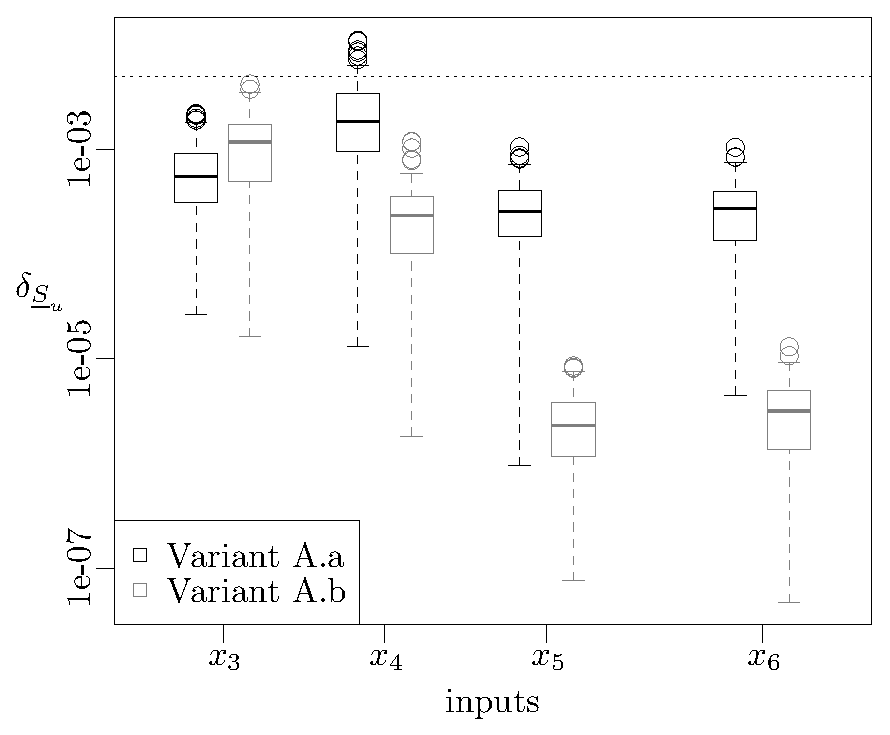
\includegraphics[width=0.45\textwidth]{sobolg_box.eps}
\label{boxplots.gfunc}
\end{figure}

As expected, we observe that the use of ``Correlation 2'' in Variant $A.b$ results in lower estimation errors for these four inputs. The discrepancy observed does not stand out in Table \ref{res.gfunc.Ab} due to its low magnitude ($10^{-4} \sim 10^{-5}$).

{\color{purple}(Lolo) Table \ref{comparison.gfunc} shows the average number of evaluations performed in Variant $A.a$ to estimate $I_1$, the numerator of $\underline{S}_u$, and $I_2$, the numerator of $\ov{$S$}_u$. The column $I_2 > I_1$ indicates the number of times where $I_2$ required more evaluations than $I_1$. We observe that $I_2$ never requires more evaluations than $I_1$. This seems to indicate that the effective dimension of $I_1$ is higher than $I_2$ for this example.
\begin{table}[t]
\caption{Number of evaluations evaluations performed to estimate $I_1$ and $I_2$ in Variant $A.a$. $N$ is the number of times among the $100$ repeats where $I_2$ required more evaluations than $I_1$}
\centering
\begin{tabular}{cccc}
\hline
 input & $I_1$ & $I_2$ & $I_2 > I_1$ \\ \hline
 $x_1$ & $32768$ & $32768$ & $0$ \\   \hline
 $x_2$ & $16384$ & $16384$ & $0$ \\  \hline
 $x_3$ & $4096$ & $2048$ & $0$ \\  \hline
 $x_4$ & $830$ & $512$ & $0$ \\  \hline
 $x_5$ & $512$ & $512$ & $0$ \\  \hline
 $x_6$ & $512$ & $512$ & $0$ \\  \hline
\end{tabular}
\label{comparison.gfunc}
\end{table}}
\bigskip

Table \ref{res.gfunc.B} shows averaged estimation errors $\delta_{\underline{S}_u}$ and total number of evaluations for Variant $B$. The results show that the use of Variant $B$ leads to slightly higher estimation errors than those obtained with Variant $A.a$ or Variant $A.b$. However, the total number of evaluations is {\color{purple}half as large}. As such, this approach remains interesting when one wants to estimate only first-order indices.
\begin{table}[t]
\caption{Averaged estimation errors $\delta_{\underline{S}_u}$ and total number of evaluations for Variant $B$.}
\centering
\begin{tabular}{cccc}
\hline
 input & $\underline{S}_u$ & $\delta_{\underline{S}_u}$ & $r_{\delta_{\underline{S}_u}}$ \\ \hline
 $x_1$ & $0.6043$ &  $0.0005$ & $0$ \\ \hline
 $x_2$ & $0.2360$ &  $0.0010$ & $0$ \\ \hline
 $x_3$ & $0.0286$ &  $0.0018$ & $0.02$ \\ \hline
 $x_4$ & $0.0043$ &  $0.0016$ & $0$    \\ \hline
 $x_5$ & $4.10^{-5}$ & $0.0034$ & $0$  \\ \hline
 $x_6$ & $4.10^{-5}$ & $0.0035$ & $0$  \\ \hline \hline
\multicolumn{4}{l}{Total number of evaluations: $65 \ 536$}\\ \hline 
\end{tabular}
\label{res.gfunc.B}
\end{table}

\subsubsection{Bratley et al. function}

In this second example, we consider the Bratley \textit{et al.} function defined by,
$$f(x_1,\dots,x_d)=\sum \limits_{i=1}^{d} (-1)^i \prod \limits_{j=1}^{i} x_j \ .$$
The importance of each variable $x_j$ depends on their own rank. More explicitly, $x_1$ is more influent than $x_2$ that is respectively more influent than $x_3$ and so on. 

As for the g-function, Tables \ref{res.bratley.Aa} and \ref{res.bratley.Ab} show averaged estimation errors and total number of evaluations for Variant $A.a$ and Variant $A.b$.
\begin{table}[!ht]
\caption{Averaged estimation errors $\delta_{\underline{S}_u}$, $\delta_{\overline{S}_u}$ and total number of evaluations for Variant $A.a$.}
\centering
\begin{tabular}{ccccccc}
\hline
 input & $\underline{S}_u$ & $\delta_{\underline{S}_u}$ & $r_{\delta_{\underline{S}_u}}$ & $\overline{S}_u$ & $\delta_{\overline{S}_u}$ &$r_{\delta_{\overline{S}_u}}$ \\ \hline
 $x_1$ & $0.6529$ &  $0.0005$ & $0$ & $0.7396$ & $0.0002$ & $0.$ \\ \hline
 $x_2$ & $0.1791$ &  $0.0006$ & $0$ & $0.2659$ & $0.0005$ & $0$ \\ \hline
 $x_3$ & $0.0370$ &  $0.0058$ & $0.78$ & $0.0764$ & $0.0015$ & $0.01$ \\ \hline
 $x_4$ & $0.0133$ &  $0.0019$ & $0.09$ & $0.0343$ & $0.0018$ & $0.02$ \\ \hline
 $x_5$ & $0.0015$ &  $0.0024$ & $0.13$ & $0.0062$ & $0.0016$ & $0.05$ \\ \hline
 $x_6$ & $0.0015$ & $0.0023$ & $0.09$  & $0.0062$ & $0.0011$ & $0$ \\ \hline \hline
\multicolumn{4}{l}{Total number of evaluations: $68 \ 404$} & & &\\ \hline 
\end{tabular}
\label{res.bratley.Aa}
\end{table}
\begin{table}[!ht]
\caption{Averaged estimation errors $\delta_{\underline{S}_u}$, $\delta_{\overline{S}_u}$ and total number of evaluations for Variant $A.b$.}
\centering
\begin{tabular}{ccccccc}
\hline
 input & $\underline{S}_u$ & $\delta_{\underline{S}_u}$ & $r_{\delta_{\underline{S}_u}}$ & $\overline{S}_u$ & $\delta_{\overline{S}_u}$ & $r_{\delta_{\overline{S}_u}}$ \\ \hline
 $x_1$ & $0.6529$ &  $0.0005$ & $0$ & $0.7396$ & $0.0002$ & $0$ \\ \hline
 $x_2$ & $0.1791$ &  $0.0006$ & $0$ & $0.2659$ & $0.0005$ & $0$ \\ \hline
 $x_3$ & $0.0370$ &  $0.0017$ & $0.02$ & $0.0764$ & $0.0015$ & $0.01$ \\ \hline
 $x_4$ & $0.0133$ &  $0.0017$ & $0$ & $0.0343$ & $0.0018$ & $0.02$ \\ \hline
 $x_5$ & $0.0015$ &  $0.0003$ & $0$ & $0.0062$ & $0.0016$ & $0.05$ \\ \hline
 $x_6$ & $0.0015$ &  $0.0004$ & $0$  & $0.0062$ & $0.0011$ & $0$ \\ \hline \hline
\multicolumn{4}{l}{Total number of evaluations: $66 \ 821$} & & &\\ \hline 
\end{tabular}
\label{res.bratley.Ab}
\end{table}

Variant $A.b$ gives lower estimation errors and fewer failure rates than Variant $A.a$ on the four small first-indices $\underline{S}_3$, $\underline{S}_4,\underline{S}_5$, $\underline{S}_6$ which highlights the performance of ``Correlation 2''. The discrepancy is particularly notable for input $x_3$ where Variant $A.a$ reaches a failure rate of $71\%$ against only $2\%$ for Variant $A.b$. Furthermore, Variant $A.b$ requires less evaluations than Variant $A.a$. The boxplots represented in Figure \ref{boxplots.bratley} emphasize the latter observations.
\begin{figure}[t]
\caption{Boxplots of estimation errors $\delta_{\underline{S}_u}$ for the four inputs $x_3,x_4,x_5,x_6$ obtained with both Variant $A.a$ and Variant $A.b$. The dashed horizontal line marks the tolerance $\varepsilon=5\cdot 10^{-3}$.}
\vspace*{0.2cm}
\centering
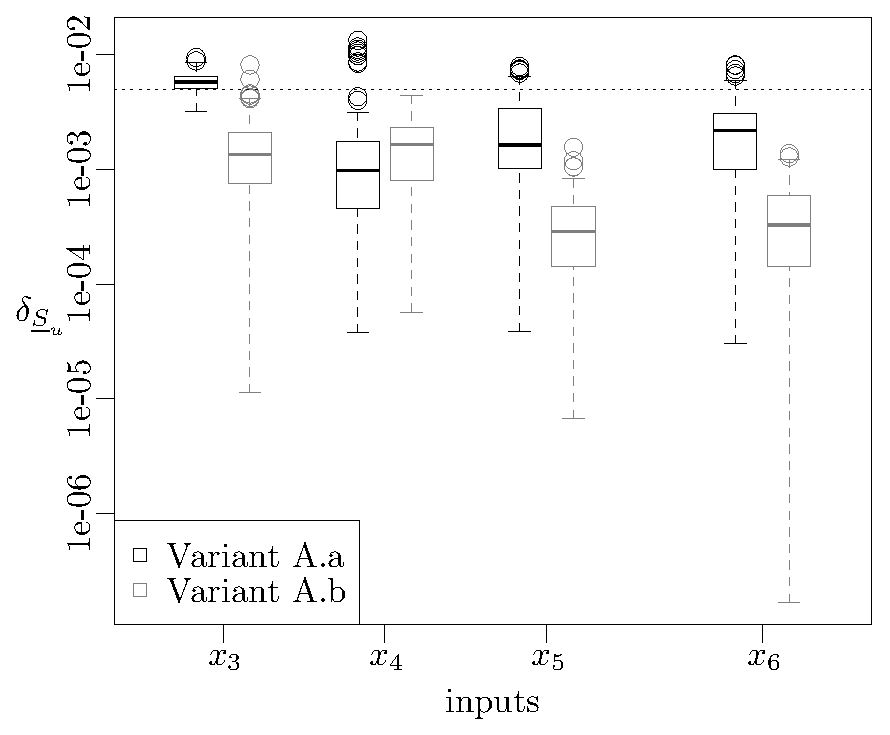
\includegraphics[width=0.45\textwidth]{bratley_box.eps}
\label{boxplots.bratley}
\end{figure}

{\color{purple}(Lolo) Table \ref{comparison.bratley} shows the average number of evaluations performed in Variant $A.a$ to estimate $I_1$, the numerator of $\underline{S}_u$, and $I_2$, the numerator of $\ov{$S$}_u$. The column $I_2 > I_1$ indicates the number of times among the $100$ repeats where $I_2$ required more evaluations than $I_1$. 
\begin{table}[t]
\caption{Number of evaluations evaluations performed to estimate $I_1$ and $I_2$ in Variant $A.a$. $N$ is the number of times where $I_2$ required more evaluations than $I_1$}
\centering
\begin{tabular}{cccc}
\hline
 input & $I_1$ & $I_2$ & $I_2 > I_1$ \\ \hline
 $x_1$ & $16876$ & $16384$ & $0$ \\  \hline
 $x_2$ & $8520$ & $8192$ & $0$ \\  \hline
 $x_3$ & $4096$ & $2786$ & $0$ \\  \hline
 $x_4$ & $3794$ & $1096$ & $4$ \\  \hline
 $x_5$ & $635$ & $512$ & $0$ \\  \hline
 $x_6$ & $712$ & $512$ & $0$ \\ 
\hline 
\end{tabular}
\label{comparison.bratley}
\end{table}
\begin{table}[t]
\caption{Averaged estimation errors $\delta_{\underline{S}_u}$ and total number of evaluations for Variant $B$.}
\centering
\begin{tabular}{cccc}
\hline
 input & $\underline{S}_u$ & $\delta_{\underline{S}_u}$ & $r_{\delta_{\underline{S}_u}}$ \\ \hline
 $x_1$ & $0.6529$ &  $0.0004$ & $0$ \\ \hline
 $x_2$ & $0.1791$ &  $0.0006$ & $0$ \\ \hline
 $x_3$ & $0.0370$ &  $0.0007$ & $0$ \\ \hline
 $x_4$ & $0.0133$ &  $0.0037$ & $0.25$    \\ \hline
 $x_5$ & $0.0015$ & $0.0023$ & $0$  \\ \hline
 $x_6$ & $0.0015$ & $0.0025$ & $0$  \\ \hline \hline
\multicolumn{4}{l}{Total number of evaluations: $65 \ 536$}\\ \hline 
\end{tabular}
\label{res.bratley.B}
\end{table}
We observe that $I_2$ almost never requires more evaluations than $I_1$. This seems to indicate that the effective dimension of $I_1$ is also higher than $I_2$ for this example.}

Table \ref{res.bratley.B} shows averaged estimation errors $\delta_{\underline{S}_u}$ and total number of evaluations for Variant $B$. The estimation errors are lower than those of Variant $A.a$ but higher than those of Variant $A.b$. Failure rates are similar to those of Variant $A.b$. Since the total number of evaluations is close to the one of Variant $A.b$ at the exception of input $x_4$. As a conclusion, Variant $B$ does not bring much improvement for this example.
\bigskip

From the results on these two test functions, the main conclusion is that Variant $A.b$ performs the best. This highlights the efficiency of ``Correlation 2'' to estimate small first-order indices with quasi-Monte Carlo methods. Even if ``Correlation 2'' originally requires more model evaluations, this drawback is overridden when this estimator is included into a sequential procedure such as ours. 

For the case where we are only interested in estimating first-order indices, Variant $B$ should be the best choice as illustrated with the g-function.

{\color{purple}
\subsection{Application}
\label{sec:5.2}

(Lolo) As an application, we will study the wing weight function introduced by Forrester \textit{et al.} \cite{Forrester} and defined as follows:
\begin{align*}
f(\vx)=0.036 x_1^{0.758} & x_2^{0.0035} \left(\frac{x_3}{\cos(x_4)^2}\right)^{0.6} x_5^{0.006} x_6^{0.04}\times \\
 & \times\left(\frac{100 x_7}{\cos(x_4)}\right)^{-0.3} (x_8 x_9)^{0.49} + x_1 x_{10}
\end{align*}
Table \ref{wing_inputs_table} gives the range of variation of each input and their physical representation.  All inputs are uniformly distributed in their respective ranges. To illustrate the performance of our procedure, five additional inert inputs $x_{11}$, $\dots$, $x_{15}$ are added which serve only to add ``noise'' to the sensitivity analysis. The inert inputs are all uniformly distributed in $[0,1]$.
\begin{table}[!ht]
\caption{Inputs and their ranges of variation. All inputs are uniformly distributed in their respective ranges.}
\centering
\begin{tabular}{ccc}
\hline
 inputs & range & description \\ \hline
$x_1$ & $[150, 200]$ & wing area (ft$^2$) \\
$x_2$ & $[220, 300]$ & weight of fuel in the wing (lb) \\
$x_3$ & $[6, 10]$ & aspect ratio \\
$x_4$ & $[-10, 10]$ & quarter-chord sweep (degrees) \\
$x_5$ & $[16, 45]$ & dynamic pressure at cruise (lb/ft$^2$) \\
$x_6$ & $[0.5, 1]$ & taper ratio \\
$x_7$ & $[0.08, 0.18]$ & aerofoil thickness to chord ratio \\
$x_8$ & $[2.5, 6]$ & ultimate load factor \\
$x_9$ & $[1700, 2500]$ & flight design gross weight (lb) \\
$x_{10}$ & $[0.025, 0.08]$ & paint weight (lb/ft$^2$) \\
$x_{11},\dots,x_{15}$ & $[0,1]$ & ``noise'' \\
\hline
\end{tabular}
\label{wing_inputs_table}
\end{table}

The motivation of this application is to test if our procedure capture the same set of influent inputs $(x_1,x_3,x_7,x_8,x_9)$ selected by the analysis of Forrester \textit{et al.}. 

A second motivation is to compare the performance of each variant ($A.a$, $A.b$ and $B$) on a function where true values of Sobol' indices cannot be computed. The comparison is based on averaged Sobol' estimates and averaged total number of evaluations over $100$ repetitions.
\bigskip


Tables \ref{res.wing.Aa}, \ref{res.wing.Ab} show the results obtained with Variant $A.a$ and  Variant $A.b$. Both variants capture well the presence of inert inputs. Variant A.b is more expansive but validates the property that first-order indices are lower or equal to total-effect indices. At the opposite, Variant A.a fails to guarantee this property for inputs with small main effects: $x_2$, $x_4$, $x_5$, $x_6$. This highlights once again the efficiency of ``Correlation 2''. The boxplots represented in Figure \ref{boxplots.wing} emphasize the latter observation, Variant $A.b$ provides less variance in the estimates. 

\begin{table}[!ht]
\caption{Averaged values of $\widehat{\underline{S}}_u$, ${\widehat{\overline{S}}_u}$, and total number of evaluations of Variant $A.a$.}
\centering
\begin{tabular}{ccc}
\hline
 input & $\widehat{\underline{S}}_u$ & $\widehat{\overline{S}}_u$ \\ \hline
 $x_1$ & $0.1245$ & $0.1279$  \\ \hline
 $x_2$ & $0.0001$ & $< 10^{-4}$  \\ \hline
 $x_3$ & $0.2203$ & $0.2261$  \\ \hline
 $x_4$ & $0.0022$ & $0.0006$  \\ \hline
 $x_5$ & $0.0011$ & $0.0001$  \\ \hline
 $x_6$ & $0.0037$ & $0.0024$  \\ \hline 
 $x_7$ & $0.1410$ & $0.1452$  \\ \hline
 $x_8$ & $0.4116$ & $0.4196$  \\ \hline
 $x_9$ & $0.0851$ & $0.0877$  \\ \hline
 $x_{10}$ & $0.0038$ & $0.0043$  \\ \hline
 $x_{11},\dots,x_{15}$ & $0$ & $0$  \\ \hline
\hline
\multicolumn{3}{l}{Total number of evaluations: $87 \ 844$} \\ \hline 
\end{tabular}
\label{res.wing.Aa}
\end{table}
\begin{table}[!ht]
\caption{Averaged values of $\widehat{\underline{S}}_u$, ${\widehat{\overline{S}}_u}$ and total number of evaluations of Variant $A.b$.}
 \centering
\begin{tabular}{ccc}
\hline
  input & $\widehat{\underline{S}}_u$ & $\widehat{\overline{S}}_u$ \\ \hline
 $x_1$ & $0.1245$ & $0.1279$  \\ \hline
 $x_2$ & $< 10^{-4}$ & $< 10^{-4}$  \\ \hline
 $x_3$ & $0.2203$ & $0.2261$  \\ \hline
 $x_4$ & $0.0006$ & $0.0006$  \\ \hline
 $x_5$ & $0.0001$ & $0.0001$  \\ \hline
 $x_6$ & $0.0023$ & $0.0024$  \\ \hline 
 $x_7$ & $0.1410$ & $0.1452$  \\ \hline
 $x_8$ & $0.4116$ & $0.4196$  \\ \hline
 $x_9$ & $0.0851$ & $0.0877$  \\ \hline
 $x_{10}$ & $0.0043$ & $0.0043$  \\ \hline
 $x_{11},\dots,x_{15}$ & $0$ & $0$  \\ \hline
\hline
\multicolumn{3}{l}{Total number of evaluations: $93 \ 881$} \\ \hline 
\end{tabular}
\label{res.wing.Ab}
\end{table}

\begin{figure}[!ht]
\caption{Boxplots of first-order indices $\underline{S}_u$ for inputs $x_2,x_4,x_5,x_6,x_{10}$ obtained with both Variant $A.a$ and Variant $A.b$.}
\vspace*{0.2cm}
\centering
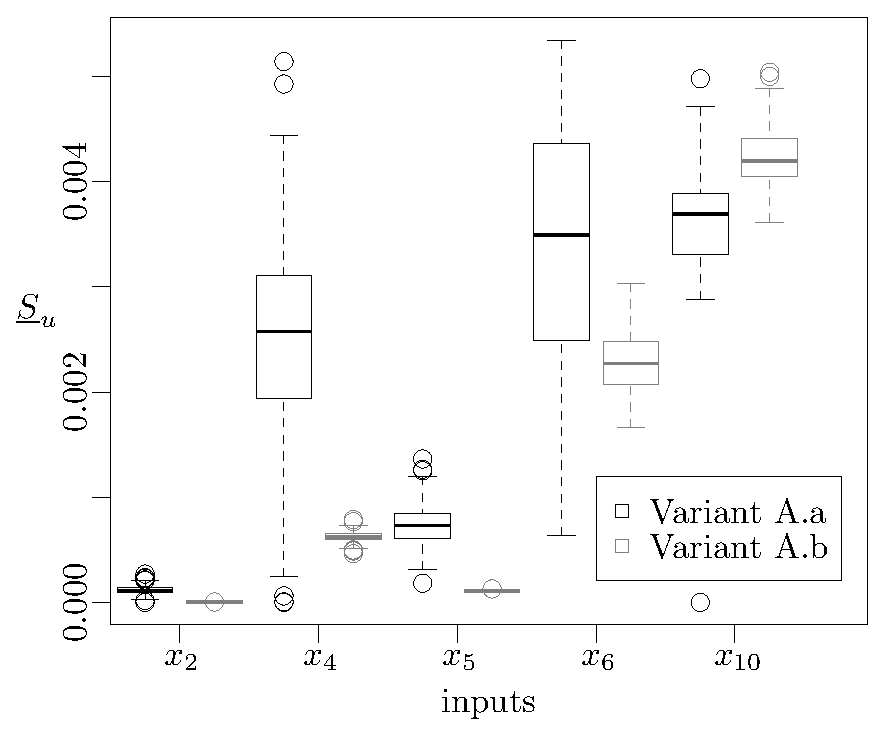
\includegraphics[width=0.45\textwidth]{wingweight_box.eps}
\label{boxplots.wing}
\end{figure}

Tables \ref{res.wing.B} show the results obtained with Variant $B$. Variant $B$ does not capture the presence of the inert inputs $x_{11}$, $\dots$, $x_{15}$. Their estimated main effects are confused with those of inputs $x_4$, $x_5$, $x_6$,$x_9$ and $x_{10}$.  However, the drawback of overestimating small first-order indices is balanced by the improvement in terms of number of evaluations. 

Overall, each variant captures well the same set of influent inputs identified by Forrester \textit{et al.}
\begin{table}[t]
\caption{Averaged values of $\widehat{\underline{S}}_u$ and total number of evaluations of Variant $B$.}
 \centering
\begin{tabular}{cc}
\hline
 input & $\widehat{\underline{S}}_u$ \\ \hline
 $x_1$ & $0.1243$ \\ \hline
 $x_2$ & $0.0035$ \\ \hline
 $x_3$ & $0.2202$ \\ \hline
 $x_4$ & $0.0033$ \\ \hline
 $x_5$ & $0.0021$ \\ \hline
 $x_6$ & $0.0037$ \\ \hline 
 $x_7$ & $0.1410$ \\ \hline
 $x_8$ & $0.4117$ \\ \hline
 $x_9$ & $0.0673$ \\ \hline
 $x_{10}$ & $0.0043$ \\ \hline
 $x_{11},\dots,x_{15}$ & $\in [6.10^{-4},7.10^{-3}]$ \\ \hline
 \hline
\multicolumn{2}{l}{Total number of evaluations: $65 \ 536$} \\ \hline 
\end{tabular}
\label{res.wing.B}
\end{table}

\subsection{Comparison with Monte Carlo method}

In this section, our procedure is compared to a simpler method based on random sampling and straightforward confidence intervals. The bratley \textit{et al.} function is used to compare both approaches. The random sampling method corresponds to Saltelli's procedure described in Section \ref{sec:2.2}. For a fair comparison, ``Correlation 2'' is used instead of \eqref{first.order.est} to estimate the small main effects of inputs $x_3$, $x_4$, $x_5$ and $x_6$. The random sampling method proceeds as follows: each Sobol' index is evaluated with the same number of evaluations used in Variant $A.b$. Then, bootstrap confidence intervals are computed. 

The results are averaged over $100$ repetitions and compared in Table \ref{compa_MC} to those obtained with Variant $A.b$. The comparison is made based on estimation errors and failures rates. The column precision corresponds to the average width of the bootstrap confidence interval for the random sampling method.

The main observation is that our procedure performs the best. The random sapling method has high failure rates for inputs $x_1$, $x_2$ and slightly worse failure rates than Variant $A.b$ for inputs $x_3$, $x_4$. The average precision only falls below the tolerance $\varepsilon=5\cdot10^{-3}$ for inputs $x_5$ and $x_6$. Figures \ref{compa_MC_first} and \ref{compa_MC_tot} emphasize the latter observations.


\begin{table}[!ht]
\caption{Averaged estimation errors $\delta_{\underline{S}_u}$, $\delta_{\overline{S}_u}$ and failure rates for the random sampling method (MC) and Variant $A.b$ (QMC).}
\centering
\begin{tabular}{ccccccc}
\hline
 input & procedure & $\delta_{\underline{S}_u}$ & $r_{\delta_{\underline{S}_u}}$ & $\delta_{\overline{S}_u}$ &$r_{\delta_{\overline{S}_u}}$ & precision \\
\hline
\multirow{2}{*}{$x_1$} & QMC & $0.0005$ & $0$ & $0.0002$ & $0$ & \multirow{2}{*}{$0.0344$} \\
& MC & $0.0116$ & $0.75$ & $0.0086$ & $0.67$ & \\
\hline
\multirow{2}{*}{$x_2$} & QMC & $0.0006$ & $0$ & $0.0005$ & $0$ & \multirow{2}{*}{$0.0362$} \\
& MC & $0.0122$ & $0.74$ & $0.0049$ & $0.37$ & \\
\hline
\multirow{2}{*}{$x_3$} & QMC & $0.0017$ & $0.02$ & $0.0015$ & $0.01$ & \multirow{2}{*}{$0.007$} \\
& MC & $0.0020$ & $0.02$ & $0.0030$ & $0.18$ & \\
\hline
\multirow{2}{*}{$x_4$} & QMC & $0.0017$ & $0$ & $0.0018$ & $0.02$ & \multirow{2}{*}{$0.0052$} \\
& MC & $0.0014$ & $0.01$ & $0.0027$ & $0.11$ & \\
\hline
\multirow{2}{*}{$x_5$} & QMC & $0.0003$ & $0$ & $0.0016$ & $0.05$ & \multirow{2}{*}{$0.0012$} \\
& MC & $0.0003$ & $0$ & $0.0011$ & $0.01$ & \\
\hline
\multirow{2}{*}{$x_6$} & QMC & $0.0004$ & $0$ & $0.0011$ & $0$ & \multirow{2}{*}{$0.0012$} \\
& MC & $0.0003$ & $0$ & $0.0010$ & $0$ & \\
\hline
\end{tabular}
\label{compa_MC}
\end{table}

\begin{figure}[!ht]
\caption{Boxplots of estimation errors $\delta_{\underline{S}_u}$ obtained with both Variant $A.b$ and the random sampling method. The dashed horizontal line marks the tolerance $\varepsilon=5\cdot 10^{-3}$.}
\centering
\vspace*{0.2cm}
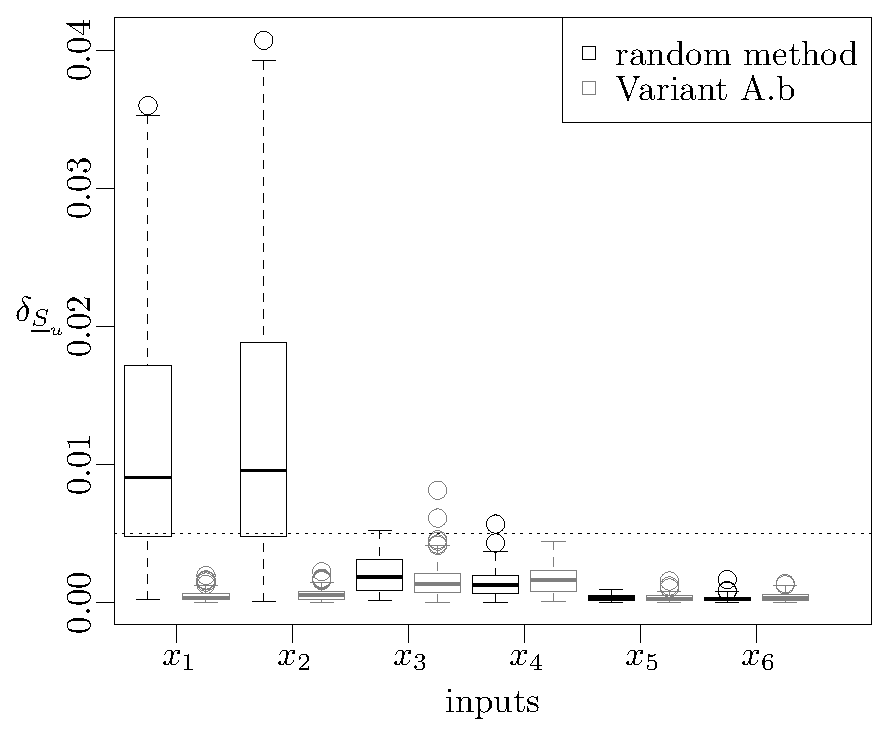
\includegraphics[width=0.4\textwidth]{comp_mc_first.eps}
\label{compa_MC_first}
\end{figure}

\begin{figure}[!ht]
\caption{Boxplots of estimation errors $\delta_{\overline{S}_u}$ obtained with both Variant $A.b$ and the random sampling method. The dashed horizontal line marks the tolerance $\varepsilon=5\cdot 10^{-3}$.}
\centering
\vspace*{0.2cm}
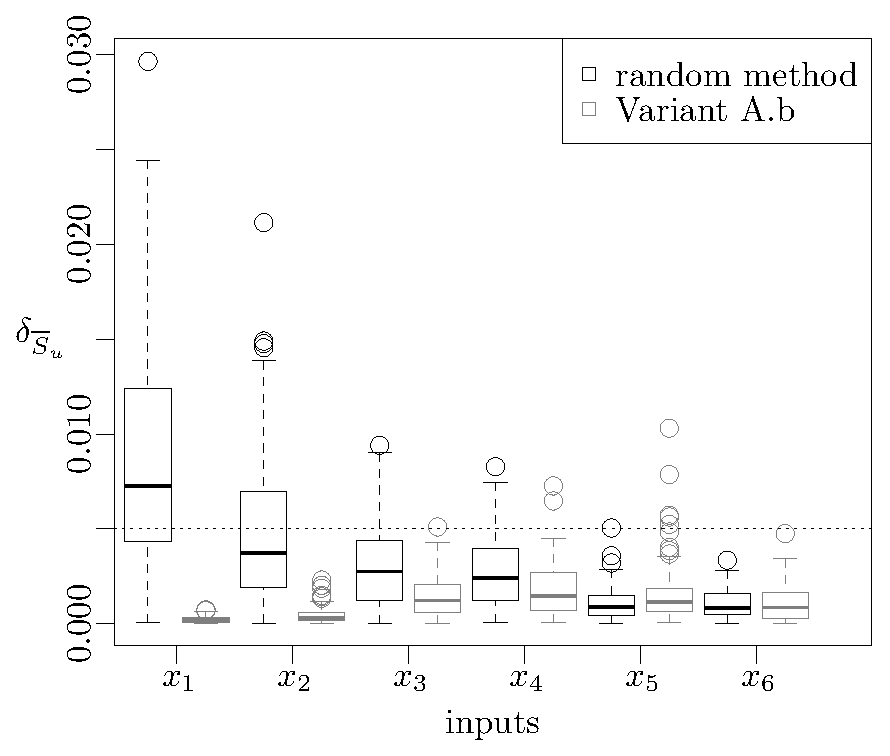
\includegraphics[width=0.4\textwidth]{comp_mc_tot.eps}
\label{compa_MC_tot}
\end{figure}}


\section{Conclusion}
When estimating Sobol' indices, the question of how many evaluations must be performed to reach a desired precision is often raised by practitioners. This question is difficult to address mostly because the number of evaluations needed depends on the complexity of the model studied. As such, it is hard to bring out a general rule of thumb. 

The sequential estimation procedure proposed in this article offers a practical solution with the construction of an estimator and error bound for Sobol' indices. The number of points is progressively augmented until the error bound becomes lower than a user specified tolerance. The procedure presented combines Sobol' sequences with either Saltelli's strategy to estimate both first-order and total effect indices, or the replication procedure to estimate only first-order indices. Furthermore, we investigated the use of a recent estimator well-suited to the estimation of small first-order indices using quasi-Monte Carlo methods. The efficiency of this estimator, called ``Correlation 2'', was assessed and highlighted on two test functions and an application. Overall, the variant combining Saltelli's strategy and ``Correlation 2'' gave the best results, with low failure rates across all indices.

{\color{purple}(Lolo) The precision of our procedure was also compared to a simpler method based on random sampling and straightforward confidence intervals. For an identical number of evaluations, our procedure was far more accurate than a random sampling method. The origin of the discrepancy observed lies in the use of a more robust error bound.}

\comment{Add that we can consider relative errors and reference ...}

As a future project, the same estimators and algorithms can be designed for rank-1 lattices using the results in \cite{JimHic}, and noticing that rank-1 lattices of the same size are also replicated designs of order 1. 

\begin{acknowledgements}
The authors thank Fred J. Hickernell and Cl\'ementine Prieur for initiating this collaborative work and Elise Arnaud for her proofreading. The authors are grateful to Stephen Joe, Frances Y. Kuo and Art B. Owen for their helpful answers and suggestions.   
\end{acknowledgements}

% BibTeX users please use one of
%\bibliographystyle{spbasic}      % basic style, author-year citations
%\bibliographystyle{spmpsci}      % mathematics and physical sciences
%\bibliographystyle{spphys}       % APS-like style for physics
%\bibliography{}   % name your BibTeX data base

% Non-BibTeX users please use
\begin{thebibliography}{99}
%
% and use \bibitem to create references. Consult the Instructions
% for authors for reference list style.
%

\bibitem{Bratley}
Bratley, P., Fox, B. L., Niederreiter, H.: Implementation and tests of low-discrepancy sequences, ACM Trans. Model. Comput. Simul. \textbf{2}(3), 195-213 (1992)
\bibitem{Forrester}
Forrester, A., S\'obester, A., Keane, A.: Engineering design via surrogate modelling, Chichester: Wiley (2008)
\bibitem{Gilquin.rec}
Gilquin, L., Arnaud, E., Monod, H., Prieur, C.: Recursive estimation procedure of Sobol' indices based on replicated designs, preprint available at \url{https://hal.inria.fr/hal-01291769}, (2016).
\bibitem{GJAHMP}
Gilquin, L., Jim\'enez Rugama, Ll. A., Arnaud, E., Hickernell, F. J., Monod, H., Prieur, C.: Iterative construction of replicated designs based on Sobol' sequences, C. R. Math., vol. 355, 10-14 (2017)
\bibitem{HicJim}
Hickernell, F. J., Jim\'enez Rugama, Ll. A.: Reliable adaptive cubature using digital sequences: Monte Carlo and Quasi-Monte Carlo Methods 2014, vol. 163, 367-383 (2016)
\bibitem{HicJimLi}
Hickernell, F. J., Jim\'enez Rugama, Ll. A., Li, D.: Adaptive quasi-Monte Carlo methods for cubature, preprint available at \url{https://arxiv.org/pdf/1702.01491.pdf}, (2017).
\bibitem{HonHic00a}
Hong, H. S., Hickernell, F. J.: Algorithm 823: Implementing scrambled digital nets, ACM Trans. Math. Software, vol. 29, 95-109, (2003)
\bibitem{Hoeffding}
Hoeffding, W. F.: A class of statistics with asymptotically normal distribution, Ann. Math. Stat. \textbf{19}(3), 293-325 (1948)
\bibitem{Janon}
Janon, A., Klein, T., Lagnoux A., Nodet, M., Prieur C.: Asymptotic normality and efficiency of two {S}obol' index estimators, ESAIM Probab. Stat. \textbf{18}, 342-364 (2014)
\bibitem{JimHic}
Jim\'enez Rugama, Ll. A., Hickernell, F. J.: Adaptive multidimensional integration based on rank-1 lattices: Monte Carlo and Quasi-Monte Carlo Methods 2014, vol. 163, 407-422 (2016)
\bibitem{Kuo} Joe, S., Kuo, F. Y., Constructing Sobol sequences with better two-dimensional projections, \emph{SIAM J. Sci. Comput.} 30(8), 2008, pp. 2635--2654.
\bibitem{Lemieuxbook}
Lemieux, C.: Monte Carlo and quasi-Monte Carlo sampling, Springer, New-York (2009)
\bibitem{Mara}
Mara, T. A., Rakoto Joseph, O.: Comparison of some efficient methods to evaluate the main effect of computer model factors, J. Statist. Comput. Simulation \textbf{78}(2), 167-178 (2008)
\bibitem{McKay}
McKay, M. D.: Evaluating prediction uncertainty, Los Alamos National Laboratory Report NUREG/CR- 6311, LA-12915-MS. (1995)
\bibitem{Niederreiter} 
Niederreiter, H.: Random number generation and quasi-Monte carlo methods: CBMS-NSF Regional Conference Series in Applied Math., vol. 63, SIAM, Philadelphia (1992)
\bibitem{Owe95}
Owen, A. B.: Randomly permuted $(t,m,s)$-nets and $(t,s)$-sequences: Monte Carlo and Quasi-Monte Carlo Methods in Scientific Computing, vol. 106, 299-317 (1995)
\bibitem{Owen}
Owen, A.B.: Better estimation of small Sobol' sensitivity indices, ACM Trans. Model. Comput. Simul. \textbf{23}(2), :11 (2013)
\bibitem{Saltelli}
Saltelli, A.: Making best use of models evaluations to compute sensitivity indices, Comput. Phys. Commun. \textbf{145}(2), 280-297 (2002)
\bibitem{Sobol'seq}
Sobol', I. M.: On the distribution of points in a cube and the approximate evaluation of integrals, USSR Comput. Math. Math. Phys. \textbf{7}(4), 86-112 (1967)
\bibitem{Sobol'}
Sobol', I. M.: Sensitivity indices for nonlinear mathematical models, Mathematical Modeling and Computational Experiment \textbf{1}, 407-414 (1993)
\bibitem{Tissot}
Tissot, J. Y., Prieur, C.: A randomized Orthogonal Array-based procedure for the estimation of first- and second-order Sobol' indices, J. Statist. Comput. Simulation \textbf{85}(7), 1358-1381 (2015)
\bibitem{Tong}
Tong, C.: Self-validated variance-based methods for sensitivity analysis of model outputs, Reliab. Eng. Syst. Saf. \textbf{95}(3), 301-309 (2010)

\end{thebibliography}
\end{document}
